%%%%%%%%%%%%%%%%%%%%%%%%%%%%%%%%%%%%%%%%%
% Journal Article
% LaTeX Template
% Version 1.4 (15/5/16)
%
% This template has been downloaded from:
% http://www.LaTeXTemplates.com
%
% Original author:
% Frits Wenneker (http://www.howtotex.com) with extensive modifications by
% Vel (vel@LaTeXTemplates.com)
%
% License:
% CC BY-NC-SA 3.0 (http://creativecommons.org/licenses/by-nc-sa/3.0/)
%
%%%%%%%%%%%%%%%%%%%%%%%%%%%%%%%%%%%%%%%%%

%----------------------------------------------------------------------------------------
%	PACKAGES AND OTHER DOCUMENT CONFIGURATIONS
%----------------------------------------------------------------------------------------

\documentclass[14pt]{article}

%\usepackage{blindtext}

\usepackage{extsizes}
\usepackage[T2A]{fontenc}
\usepackage[utf8]{inputenc}
\usepackage[english, russian]{babel}

%\usepackage{times}
\linespread{1.5}

\usepackage[left=3cm,right=1cm,top=1.5cm,bottom=2cm]{geometry}
\usepackage[framed,numbered,autolinebreaks,useliterate]{mcode}

\usepackage{graphicx, amsmath}
\numberwithin{figure}{section}
\graphicspath{{images/}}
\usepackage{amsfonts}

\numberwithin{equation}{section}

\usepackage{booktabs} % Horizontal rules in tables

\usepackage{lettrine} % The lettrine is the first enlarged letter at the beginning of the text

\usepackage{enumitem} % Customized lists
\setlist[itemize]{noitemsep} % Make itemize lists more compact

\usepackage{listings}
\lstloadlanguages{C,[ANSI]C++}%,Clean,make,Fortran}%Загружаемые языки
\lstset{
  language=C,                % choose the language of the code
  numbers=left,                   % where to put the line-numbers
  stepnumber=1,                   % the step between two line-numbers.
  numbersep=5pt,                  % how far the line-numbers are from the code
  backgroundcolor=\color{white},  % choose the background color. You must add \usepackage{color}
  showspaces=false,               % show spaces adding particular underscores
  showstringspaces=false,         % underline spaces within strings
  showtabs=false,                 % show tabs within strings adding particular underscores
  tabsize=2,                      % sets default tabsize to 2 spaces
  captionpos=b,                   % sets the caption-position to bottom
  breaklines=true,                % sets automatic line breaking
  breakatwhitespace=true,         % sets if automatic breaks should only happen at whitespace
  %title=\lstname,                 % show the filename of files included with \lstinputlisting;
}

\usepackage{abstract} % Allows abstract customization
\renewcommand{\abstractnamefont}{\normalfont\bfseries} % Set the "Abstract" text to bold
\renewcommand{\abstracttextfont}{\normalfont\small\itshape} % Set the abstract itself to small italic text

%\usepackage{titlesec} % Allows customization of titles
% \renewcommand\thesection{\Roman{section}} % Roman numerals for the sections
% \renewcommand\thesubsection{\roman{subsection}} % roman numerals for subsections
% \titleformat{\section}[block]{\large\scshape\centering}{\thesection.}{1em}{} % Change the look of the section titles
% \titleformat{\subsection}[block]{\large}{\thesubsection.}{1em}{} % Change the look of the section titles

\usepackage{titling} % Customizing the title section

\usepackage{hyperref} % For hyperlinks in the PDF
\usepackage{setspace}
\onehalfspacing

%----------------------------------------------------------------------------------------
%	TITLE SECTION
%----------------------------------------------------------------------------------------


%----------------------------------------------------------------------------------------

\begin{document}
\begin{titlepage}

\thispagestyle{empty}
\newgeometry{margin=2cm}
\center
\textsc{МИНОБРНАУКИ РОССИИ}\\
\textbf{ФЕДЕРАЛЬНОЕ ГОСУДАРСТВЕННОЕ БЮДЖЕТНОЕ ОБРАЗОВАТЕЛЬНОЕ УЧРЕЖДЕНИЕ ВЫСШЕГО ОБРАЗОВАНИЯ\\<<ВОРОНЕЖСКИЙ ГОСУДАРСТВЕННЫЙ УНИВЕРСИТЕТ>>}

\vspace{0.3cm}

\centerline{Факультет компьютерных наук}
\centerline{Кафедра цифровых технологий}

\vspace{1cm}

\centerline{Применение сверточных нейронных сетей к задаче }
\centerline{классификации трехмерных моделей}

\vspace{1cm}

\centerline{ВКР Бакалаврская работа}
\centerline{02.03.01 Математика и компьютерные науки}
\centerline{Распределенные системы и искусственный интеллект}

\vfill
\begin{flushleft}
\textrm{Допущено к защите в ГЭК \rule[0mm]{5mm}{0,3mm} . \rule[0mm]{15mm}{0,3mm} . 2017}
\end{flushleft}
\begin{tabbing}
ооооооооооооооо	\=	----------------------	\kill
Зав. кафедрой	\> 	\rule[0mm]{4cm}{0,3mm}	\textit{С.Д. Кургалин, д. ф.-м. н., профессор} \\
Обучающийся 	\> 	\rule[0mm]{4cm}{0,3mm}	\textit{А.А. Вакулин, 4 курс, д/о}             \\
Руководители	\> 	\rule[0mm]{4cm}{0,3mm}  \textit{А.А. Крыловецкий, к. ф.-м. н., доцент} \\
				\> 	\rule[0mm]{4cm}{0,3mm}  \textit{И.С. Черников, к. ф.-м. н., ассистент}
\end{tabbing}

\vfill

\centerline{Воронеж 2017}
\clearpage
\end{titlepage}

%----------------------------------------------------------------------------------------
%	ARTICLE CONTENTS
%----------------------------------------------------------------------------------------

%% ЗАДАНИЕ НА ВЫПОЛНЕНИЕ
\newpage\thispagestyle{empty}
\addtocounter{page}{1}
\newgeometry{margin=2cm}
\begin{spacing}{1.2}
{
\begin{center}
{\small МИНОБРНАУКИ РОССИИ}\\  \!  \!  \!
{\small \textbf{ФЕДЕРАЛЬНОЕ ГОСУДАРСТВЕННОЕ БЮДЖЕТНОЕ}}\\ \!  \!  \!
{\small \textbf{ОБРАЗОВАТЕЛЬНОЕ УЧРЕЖДЕНИЕ}}\\ \!  \!
{\small  \textbf{ВЫСШЕГО ОБРАЗОВАНИЯ}\\ \!  \!
\textbf{''ВОРОНЕЖСКИЙ ГОСУДАРСТВЕННЫЙ УНИВЕРСИТЕТ''}\\ \!  \!
Факультет компьютерных наук\\  \!  \! \!
$~$Кафедра цифровых технологий}\\
\vspace{0.1cm}
\end{center}
\begin{flushright} \!  \!  \! \!
{\small \textbf{УТВЕРЖДАЮ}\\
заведующий кафедрой\\
 $\underset{\text{\emph{подпись}}}{\underline{\hspace{0.15\textwidth}}}$ $\underset{\text{\emph{расшифровка подписи}}}{\underline{\hspace{0.3\textwidth}}}$}
\end{flushright}
\begin{center}
{\small \textbf{ЗАДАНИЕ \\
НА ВЫПОЛНЕНИЕ ВЫПУСКНОЙ КВАЛИФИКАЦИОННОЙ РАБОТЫ\\
ОБУЧАЮЩЕГОСЯ} $\underset{\text{\emph{фамилия, имя, отчество}}}{\underline{\hspace{0.69\textwidth}}}$}
\end{center}\! \! \!
\vspace{0.1cm}
{\small 1. Тема работы \underline{\phantom{aaaaaaaaaaaaaaaaaaaaaaaaaaaaaaaaaaaaaaaaaaaaaa}}, утверждена решением ученого совета \underline{\phantom{aaaaaaaaaaaaaaaaaaaaaaa}} факультета от \underline{\phantom{aaa}}.\underline{\phantom{aaa}}.20\underline{\phantom{aaa}}\\
2. { Направление подготовки $\underset{\text{\emph{шифр, наименование}}}{\underline{\hspace{0.67\textwidth}}}$\\
3. Срок сдачи студентом законченной работы \underline{\phantom{aaa}}.\underline{\phantom{aaa}}.20\underline{\phantom{aaa}}\\
4. Календарный план:}\\
\begin{tabular}[t]{|p{3em}|p{20em}|p{13em}|}
\hline
{\small	№} & {\small	Задание} & {\small Срок выполнения }\\
\hline
	{\small	$1$} & {} & {} \\
\hline
	{\small	$2$} & {} & {} \\
\hline
	{\small	$3$} &{} & {} \\
\hline
	{\small	$4$} &{} & {} \\
\hline
	{\small	$5$} &{} & {} \\
\hline
	{\small	$6$} &{} & {} \\
\hline
\end{tabular}\! \! \! \!
\begin{flushleft}
\vspace{0.4cm}
{\small
Обучающийся $~~~~~~~~\underset{\text{\emph{подпись}}}{\underline{\hspace{0.2\textwidth}}}$ $\underset{\text{\emph{расшифровка подписи}}}{\underline{\hspace{0.4\textwidth}}}$\\
\vspace{0.4cm}
Руководитель $~~~~~~~~\underset{\text{\emph{подпись}}}{\underline{\hspace{0.2\textwidth}}}$ $\underset{\text{\emph{расшифровка подписи}}}{\underline{\hspace{0.4\textwidth}}}$}
\end{flushleft}\! \! \! \! \! \! \! \!
\begin{flushleft}
\underline{\phantom{a}} \underline{\phantom{a}} \underline{\phantom{a}} \underline{\phantom{a}} \underline{\phantom{a}} \underline{\phantom{a}} \underline{\phantom{a}} \underline{\phantom{a}} \underline{\phantom{a}} \underline{\phantom{a}} \underline{\phantom{a}} \underline{\phantom{a}} \underline{\phantom{a}} \underline{\phantom{a}} \underline{\phantom{a}} \underline{\phantom{a}} \underline{\phantom{a}} \underline{\phantom{a}} \underline{\phantom{a}} \underline{\phantom{a}} \underline{\phantom{a}} \underline{\phantom{a}} \underline{\phantom{a}} \underline{\phantom{a}} \underline{\phantom{a}} \underline{\phantom{a}} \underline{\phantom{a}} \underline{\phantom{a}} \underline{\phantom{a}} \underline{\phantom{a}}
\underline{\phantom{a}} \underline{\phantom{a}} \underline{\phantom{a}} \underline{\phantom{a}} \underline{\phantom{a}} \underline{\phantom{a}} \underline{\phantom{a}} \underline{\phantom{a}} \underline{\phantom{a}} \underline{\phantom{a}} \underline{\phantom{a}} \underline{\phantom{a}} \underline{\phantom{a}} \underline{\phantom{a}} \underline{\phantom{a}} \underline{\phantom{a}} \underline{\phantom{a}} \underline{\phantom{a}} \underline{\phantom{a}}
\end{flushleft}\! \! \! \!
{\small
Выпускная квалификационная работа представлена на кафедру \underline{\phantom{aaa}}.\underline{\phantom{aaa}}.20\underline{\phantom{aaa}}\\
Рецензент $\underset{\text{\emph{должность, ученая степень, ученое звание}}}{\underline{\hspace{0.9\textwidth}}}$\\
Выпускная квалификационная работа на тему {\underline{\hspace{0.5\textwidth}}}\\
{\underline{\hspace{1\textwidth}}}\\
допущена к защите в ГЭК \underline{\phantom{aaa}}.\underline{\phantom{aaa}}.20\underline{\phantom{aaa}}\\
Заведующий кафедрой $\underset{\text{\emph{подпись, расшифровка подписи}}}{\underline{\hspace{0.4\textwidth}}}$  \underline{\phantom{aaa}}.\underline{\phantom{aaa}}.20\underline{\phantom{aaa}}\\
}
}}
\end{spacing}

%% РЕФЕРАТ
\newpage\thispagestyle{empty}
\begin{center}
РЕФЕРАТ
\end{center}

\begin{flushleft}
Бакалаврская работа  с.,  источника,  приложения\\
\vspace{0.5cm}

\vspace{0.5cm}
Объект исследования "--- \\
\vspace{0.5cm}
Цель работы "--- \\
\vspace{0.5cm}
Метод исследования и аппаратура "---\\
\vspace{0.5cm}

Полученные результаты и их новизна "---\\
\vspace{0.5cm}
Область применения "---\\
\vspace{0.5cm}
Прогнозные предположения о развитии объекта исследования "---.
\end{flushleft}

\normalsize
\newgeometry{top=15mm, left=30mm, right=15mm, bottom=20mm}

%\newpage

% \pagestyle{plain} % нумерация вкл.
% \setcounter{page}{2} % начать нумерацию с номера два
\tableofcontents

\newpage

\section*{Введение}
\addcontentsline{toc}{section}{Введение}

Трёхмерное компьютерное зрение является одной из быстро развивающихся подобластей компьютерного зрения. Это связано, прежде всего, с тем, что лишь совсем недавно появились вычислительные мощности, способные справиться с обработкой крупных объёмов трёхмерных данных. Кроме того, в настоящее время непрерывно увеличивается количество доступных трёхмерных моделей в сети Интернет, а также в специализированных базах данных.%+
Работы по созданию программно-аппаратных комплексов для получения пространственных данных объектов реального мира и воссоздания (реконструкции) точных трёхмерных моделей успешно ведутся лабораторией Stanford Computer
Graphics Laboratory (Стэнфорд, США), а также компанией DAVID Vision Systems GmbH (Кобленц, Германия). Модели поиска трёхмерных моделей в крупных базах данных разрабатываются в лабораториях Center for Geometry,
Imaging and Virtual Environments (Утрехт, Нидерланды), Laboratoire d'Informatique Fondamentale de Lille (Вильнёв-д’Аск, Франция), Microsoft Research Cambridge (Кембридж, Великобритания), Princeton Shape Retrieval
and Analysis Group(Принстон, США).%+

Здесь возникает потребность классификации моделей для дальнейшего их распознавания или поиска, а именно разработка соответствующей системы обработки баз данных трехмерных моделей.%+
Разработкой методов и алгоритмов реконструкции и поиска трёхмерных моделей занимаются учёные всего мира: P. Min, M. Kazhdan, S. Rusinkiewicz (Принстон, США), R.C. Veltkamp (Утрехт, Нидерланды), Chi-Chou Kao (Тайнань, Тайвань), группа под управлением Dr.-Ing. Simon Winkelbach (Брауншвейг, Германия).%+

Центральной проблемой, возникающей при классификации или поиске в базах данных, содержащих трехмерные объекты, является разработка метода сравнения трёхмерных моделей. В данной работе представлена реализация подобного метода, состоящая из двух основных этапов: построение дескрипторов трехмерных моделей и сравнение их между собой.

На первом этапе информацию о форме поверхности трёхмерных полигональных моделей следует представить в достаточно сжатом и ёмком виде. Это продиктовано тем, что модели имеют разный масштаб, по-разному ориентированы и локализованы в пространстве, что делает невозможным непосредственное сравнение трехмерных моделей. Удачным способом такого представления модели является ее глобальный дескриптор в виде интегрального спинового изображения\cite{Chernikoff}. Классификация таких дескрипторов трехмерных моделей требует сравнения интегральных спиновых изображений, представляющих собой массив пикселей, а не структур, описывающих трехмерные объекты.

Однако при более детальном рассмотрении поставленной задачи, в дальнейшем станет понятно, что интегральное спиновое изображение способно хранить информацию о форме поверхности только если целевая полигональная модель имеет определенное разрешение(среднюю длину ребра между точками). Алгоритм контроля разрешения трехмерных моделей также будет рассмотрен в данной работе.

После построения дескриптора трехмерной модели возникает второй этап представленного метода. Сравнение двух интегральных спиновых изображений довольно сложная задача, т.к. выделить какой-либо отличительный признак для определенного класса объектов из данных массивов на первый взгляд практически невозможно. Достаточно эффективным инструментом определения более сложных признаков из сырых массивов пикселов в настоящий момент является отдельный тип нейронных сетей, называемых свёрточными.%+
В настоящий момент над задачей распознавания трехмерных объектов с помощью нейронных сетей работают ученые из Стэнфорда, Принстона и Мюнхенского технического университета. Создаются обширные открытые библиотеки доступных аннотированных 3D-данных такие как ScanNet или The Princeton Shape Benchmark, которые, в свою очередь, будут использоваться для обучения нейронных сетей.%+

В работе будут подробнее рассмотрены оба этих этапа и приведены результаты применения данного метода для небольшой базы данных трехмерных моделей.

\section{Глобальные дескрипторы поверхности}

\subsection{Дескрипторы формы поверхности}

Понятие дескрипторов формы поверхности можно определить, как отображение пространства трёхмерных моделей в некоторое многомерное конечное векторное пространство.

Формирование отображения, сохраняющего наибольшее количество информации о поверхности модели и при этом формирующего вектор соответствующих параметров наименьшей размерности, является основной целью разработки дескрипторов поверхности. Так же дескриптор формы поверхности должен быть инвариантен относительно таких преобразований, как трансляция, вращение и масштабирование. Таким образом он будет одинаково описывать модель вне зависимости от её масштаба, положения и ориентации в пространстве. Соответствие последним требованиям зачастую может быть достигнуто предварительной обработкой данных трёхмерной модели.

% В течении последних двух десятилетий в процессе решения различных задач трёхмерного компьютерного зрения было разработано множество различных дескрипторов поверхности. Ниже, на рис.\ref{ris:1} схематически представлены некоторые разновидности используемых дескрипторов.
%
% \begin{figure}[h]
% 	\begin{center}
% 		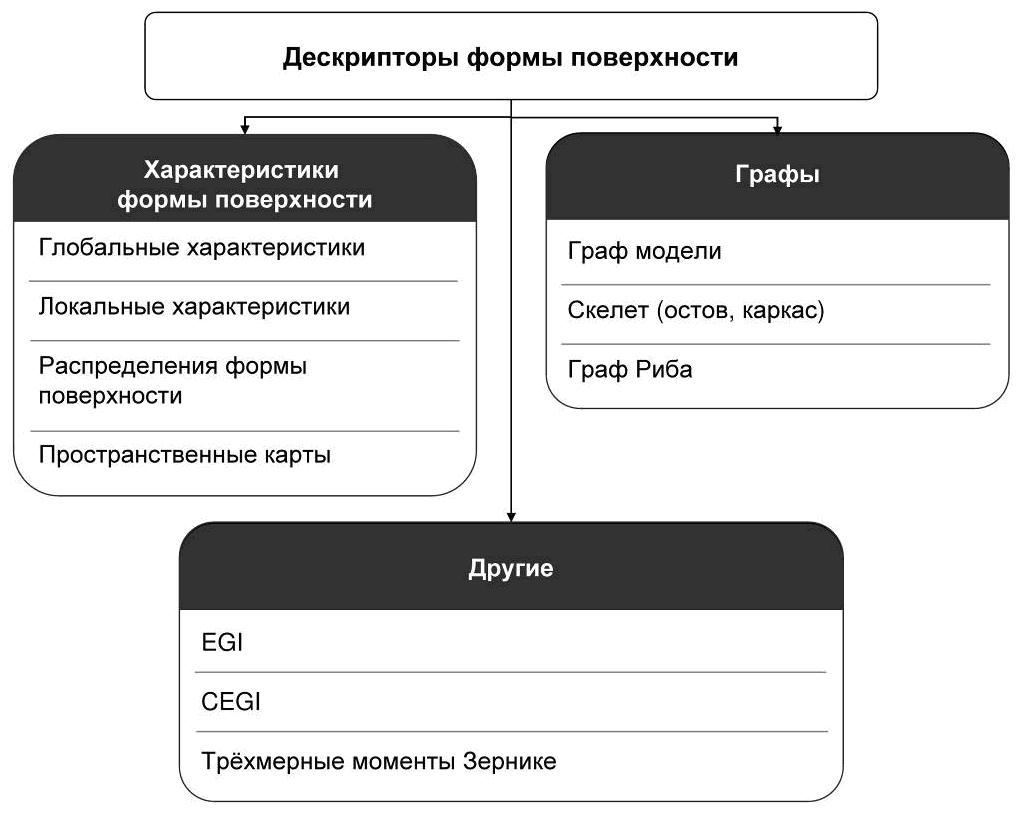
\includegraphics[scale=0.55]{1.JPG}
% 		\caption{Разновидности дескрипторов формы поверхности: граф (слева), гистограмма (внизу), спиновое изображение (справа)}
% 		\label{ris:1}
% 	\end{center}
% \end{figure}

Дескрипторы формы поверхности возможно разделить на три основных класса рис.\ref{ris:1}: характеристики формы, графы и другие. Данные категории достаточно взаимосвязаны и не являются изолированными. Таким образом, дескрипторы, основанные на распределениях, содержат глобальные характеристики формы поверхности, а дескрипторы-гистограммы могут рассматриваться как дескрипторы, основанные на методе пространственных карт. Так же, например, графы могут восприниматься как глобальные характеристики формы поверхности.

\begin{figure}[h]
	\begin{center}
		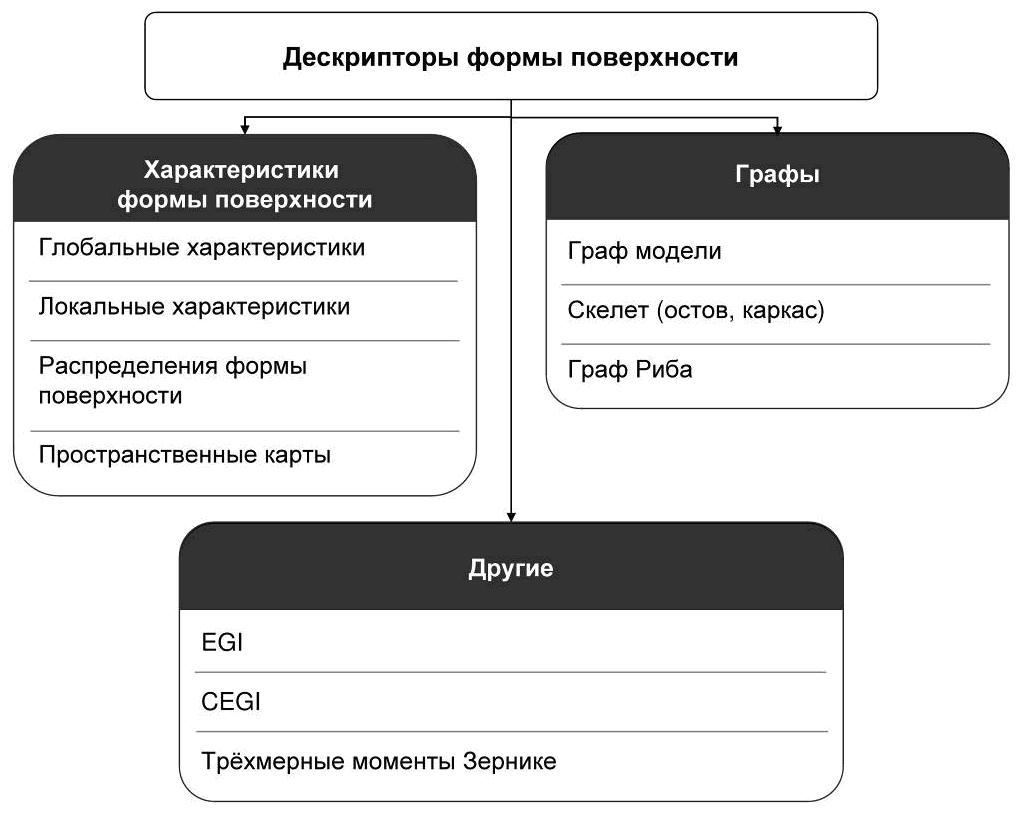
\includegraphics[scale=0.46]{1.JPG}
		\caption{Классификация дескрипторов формы поверхности}
		\label{ris:1}
	\end{center}
\end{figure}

С точки зрения сравнения трёхмерных моделей их характеристиками служат геометрические и топологические свойства их поверхности. Таким образом, измерение и сравнении этих характеристик определяет сходство или различие рассматриваемых моделей.

Для методов, базирующихся на характеристиках формы поверхности, можно выделить четыре подгруппы, которые различаются типами характеристик формы: глобальные характеристики, локальные характеристики, распределения и пространственные карты. Исключая локальные характеристики, во всех остальных подгруппах данного класса форма поверхности трёхмерных моделей описывается единственным дескриптором, который представляет собой n-мерный вектор значений. Заметим, что размерность этого вектора фиксирована для всех моделей. В методе, который основан на локальных характеристиках, дескрипторы вычисляются для всех точек поверхности модели. Таким образом каждый дескриптор содержит информацию о форме небольшого участка поверхности модели.

К другим дескрипторам отнесем расширенное Гауссово изображение (Extended Gaussian Image (EGI)) \cite{Horn}, сложное расширенное Гауссово изображение (complex EGI) \cite{Kang}, трёхмерные моменты Зернике \cite{Novotni} и др.

\subsection{Спиновые изображения}

Основная идея спиновых изображений - это сопоставление опорной точке (точке поверхности, для которой вычисляется локальный дескриптор) цилиндрической системы координат без учёта полярного угла. Опорная точка в этом случае принимается за начало системы координат, а ось $z$ расположена вдоль вектора нормали к поверхности в опорной точке. Теперь поставим в соответствие координатам $\rho$ и $z$ цилиндрической системы координат две относительные координаты спинового изображения $\alpha$ и $\beta$, как показано на рис.\ref{ris:2}. Так как полярный угол $\varphi$ цилиндрической системы координат в данном случае не учитывается, спиновое изображение получается инвариантно относительно преобразования вращения.

\begin{figure}[h]
	\begin{center}
		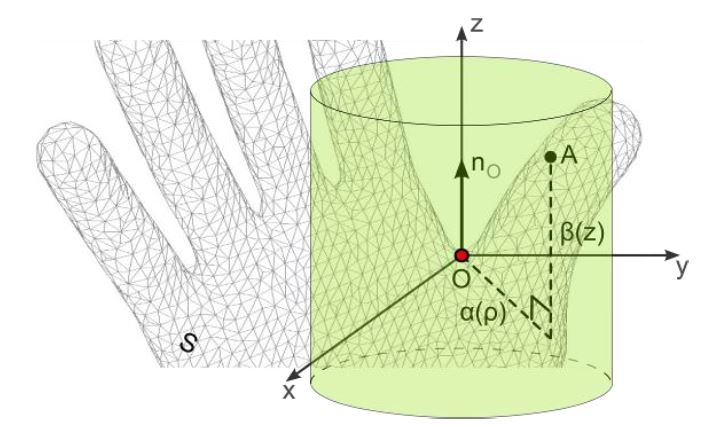
\includegraphics[scale=0.9]{2.JPG}
		\caption{Относительные координаты спинового изображения $\alpha$ и $\beta$}
		\label{ris:2}
	\end{center}
\end{figure}

%нр
Отсюда можно сделать вывод, что точки с одинаковыми значениями $\alpha$ и $\beta$ лежат на окружности радиуса $\alpha$ и на расстоянии $\beta$ от точки $O$ вдоль её нормали. На практике точек с абсолютно одинаковыми значениями $\alpha$ и $\beta$, как правило, не существует. Поэтому значения $\alpha$ и $\beta$ разбивают на классы (корзины) и подсчитывают количество точек поверхности, попавших в каждый класс.

Таким образом, для вычисления спинового изображения используются точки поверхности $S$, ограниченные цилиндром с центром в точке $O$, высотой $\beta_{max} = W_{\beta}b_{\beta}$ и радиусом $\alpha_{max} = W_{\alpha} b_{\alpha}$. В случае спиновых изображений корзины имеют форму трёхмерных колец как показано на рис.\ref{ris:3}.
%нр-

\begin{figure}[h]
	\begin{center}
		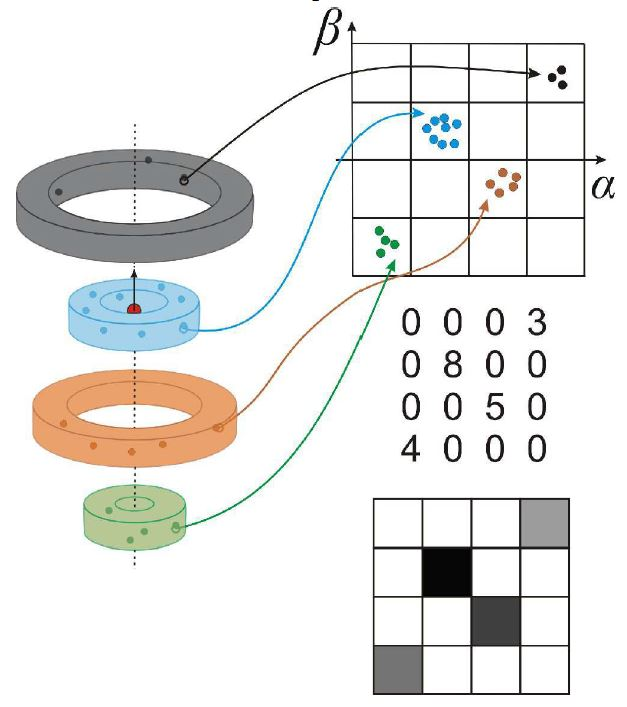
\includegraphics[scale=0.7]{3.JPG}
		\caption{Корзины спинового изображения}
		\label{ris:3}
	\end{center}
\end{figure}


Зависимость между значениями относительных координат спинового изображения $\alpha$, $\beta$ и целочисленными координатами (индексами) $i$, $j$ корзин $M_O[i, j]$ приведена ниже:

\begin{equation}
	i = \left[ \frac{\frac{W_{\beta}}{2} - \beta}{b_{\beta}} \right], \qquad j = \left[ \frac{\alpha}{b_{\alpha}} \right]
\end{equation}

\subsection{Интегральные спиновые изображения в качестве \\ глобальных дескрипторов поверхности}

Понятие глобального дескриптора поверхности можно определить, как вектор параметров, описывающий геометрию поверхности трёхмерной модели в компактной и информативной форме. Данное представление двух трехмерных моделей удобно использовать для их сравнения.

В данной работе, для сравнения формы моделей предлагается использовать интегральные спиновые изображения в качестве глобальных дескрипторов поверхности. Конкретнее, интегральным спиновым изображением, в нашем случае, будет являться, рассмотренный ранее, локальный дескриптор поверхности - спиновое изображение, вычисленный для всей модели сразу. Таким образом, понятие интегрального спинового изображения является расширением понятия обычных спиновых изображения, пригодным для описания формы всей поверхности модели.
Выбор интегральных спиновых изображений в качестве глобальных дескрипторов поверхности обусловлен их хорошими описательными характеристиками, достаточной простотой вычисления, а также устойчивостью к наличию шумов.

Очевидно, что для вычисления обычного спинового изображения необходимо знание координат опорной точки и вектора нормали к поверхности модели в этой точке. При этом опорной точкой принимается одна из точек модели. При построении же глобального дескриптора интегрального спинового изображения выбор опорной точки и вектора нормали представляет собой более сложную задачу. Это обусловлено, например, тем, что глобальные дескрипторы поверхности, вычисленные для идентичных моделей, должны быть совершенно одинаковыми даже если они по-разному ориентированы в пространстве.

В качестве опорной точки предлагается выбрать, так называемый, центр модели. Определим его как среднее арифметическое координат точек модели. Также для нахождения опорного вектора, необходимо, чтобы центр модели был расположен в начале системы координат. Для этого нужно преобразовать модель таким образом, чтобы среднее арифметическое точек модели стало равным нулю. Данное преобразование достигается смещением всех точек модели в соответствии с вектором трансляции $t$, который находится по формуле:

\begin{equation}
	t = \frac{\sum\limits^{n}_{i = 1} p_i}{n},
\end{equation}

где $p_i \in \mathbb{R}^3$ - координаты точек трехмерной модели, $n$ - количество точек трехмерной модели.

Для выбора вектора нормали предлагается использовать метод уменьшения размерности системы – метод главных компонент PCA описанный в работе \cite{Chernikoff}.

Точки, формирующие дескриптор, ограничены некоторой окрестностью опорной точки спинового изображения. В случае интегральных спиновых изображений, все точки трёхмерной модели должны быть учтены при построении глобального дескриптора. Естественно, что параметры генерации (размер корзин и ширина) интегрального спинового изображения должны оставаться постоянными для всех моделей.
%нр
Проблема попадания всех точек трёхмерной модели в окрестность опорной точки решается путём оптимального масштабирования трёхмерных моделей и дальнейшей нормализации (масштабировании) интегральных спиновых изображений. Ещё одна проблема, приводящая к ошибкам сравнения трёхмерных моделей, связана с неравномерным распределением точек модели по поверхности (то есть в одной части поверхности модели точки могут быть расположены тесно, а в другой они могут быть сильно разрежены) рис.\ref{ris:4}. Другими словами, разрешение трёхмерной модели (средняя длина рёбер, соединяющих точки модели) может значительно различаться на разных участках поверхности модели. Проблема разрешения трехмерной модели играет очень важную роль в процессе построения дескрипторов и их сравнения. Подробнее эта тема обсуждается в следующем разделе.

\begin{figure}[h]
	\begin{center}
		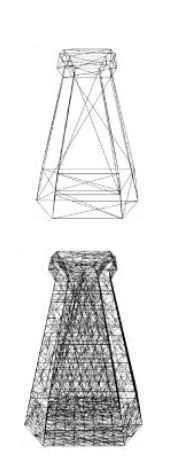
\includegraphics[scale=0.9]{4.JPG}
		\caption{Верхнее изображение – трёхмерная модель с неравномерным распределением точек; нижнее изображение – та же модель с унифицированным разрешением}
		\label{ris:4}
	\end{center}
\end{figure}

Интегральное спиновое изображение вычисляется аналогично схеме для обычного спинового изображения, за исключением того, что используемые специфические опорная точка и вектор, а также окрестность опорной точки выбираются таким образом, чтобы абсолютно все точки модели попали в неё. За счёт вычисления относительных координат $\alpha$ и $\beta$ для всех точек модели интегральное спиновое изображение описывает форму всей поверхности модели. Преимуществами использования идеи спиновых изображений при построении глобальных дескрипторов поверхности являются их хорошие описательные характеристики, относительно небольшие вычислительные затраты на их построение и обработку, а также наличие эффективного и простого метода их сравнения.
%нр-
\newpage

\section{Алгоритм контроля разрешения трехмерных \\ объектов}\label{sect2}

\subsection{Определения}

Как уже было сказано ранее, неравномерное распределение точек модели по поверхности значительно влияет на вид интегрального спинового изображения и, как следствие, приводит к ошибкам сравнения дескрипторов. Более того, модели, состоящие из малого количества точек, не позволяют построить спинового изображения, которое бы явно выделяло его признаки. На рис.\ref{ris:5} представлена одна и та же модель, но с разными средними длинами ребер, а также глобальные дескрипторы для каждого случая. Совершенно очевидно, что никаких отличительных признаков для модели с малым количеством точек и длинными ребрами выявить невозможно.

\begin{figure}[h]
	\begin{center}
		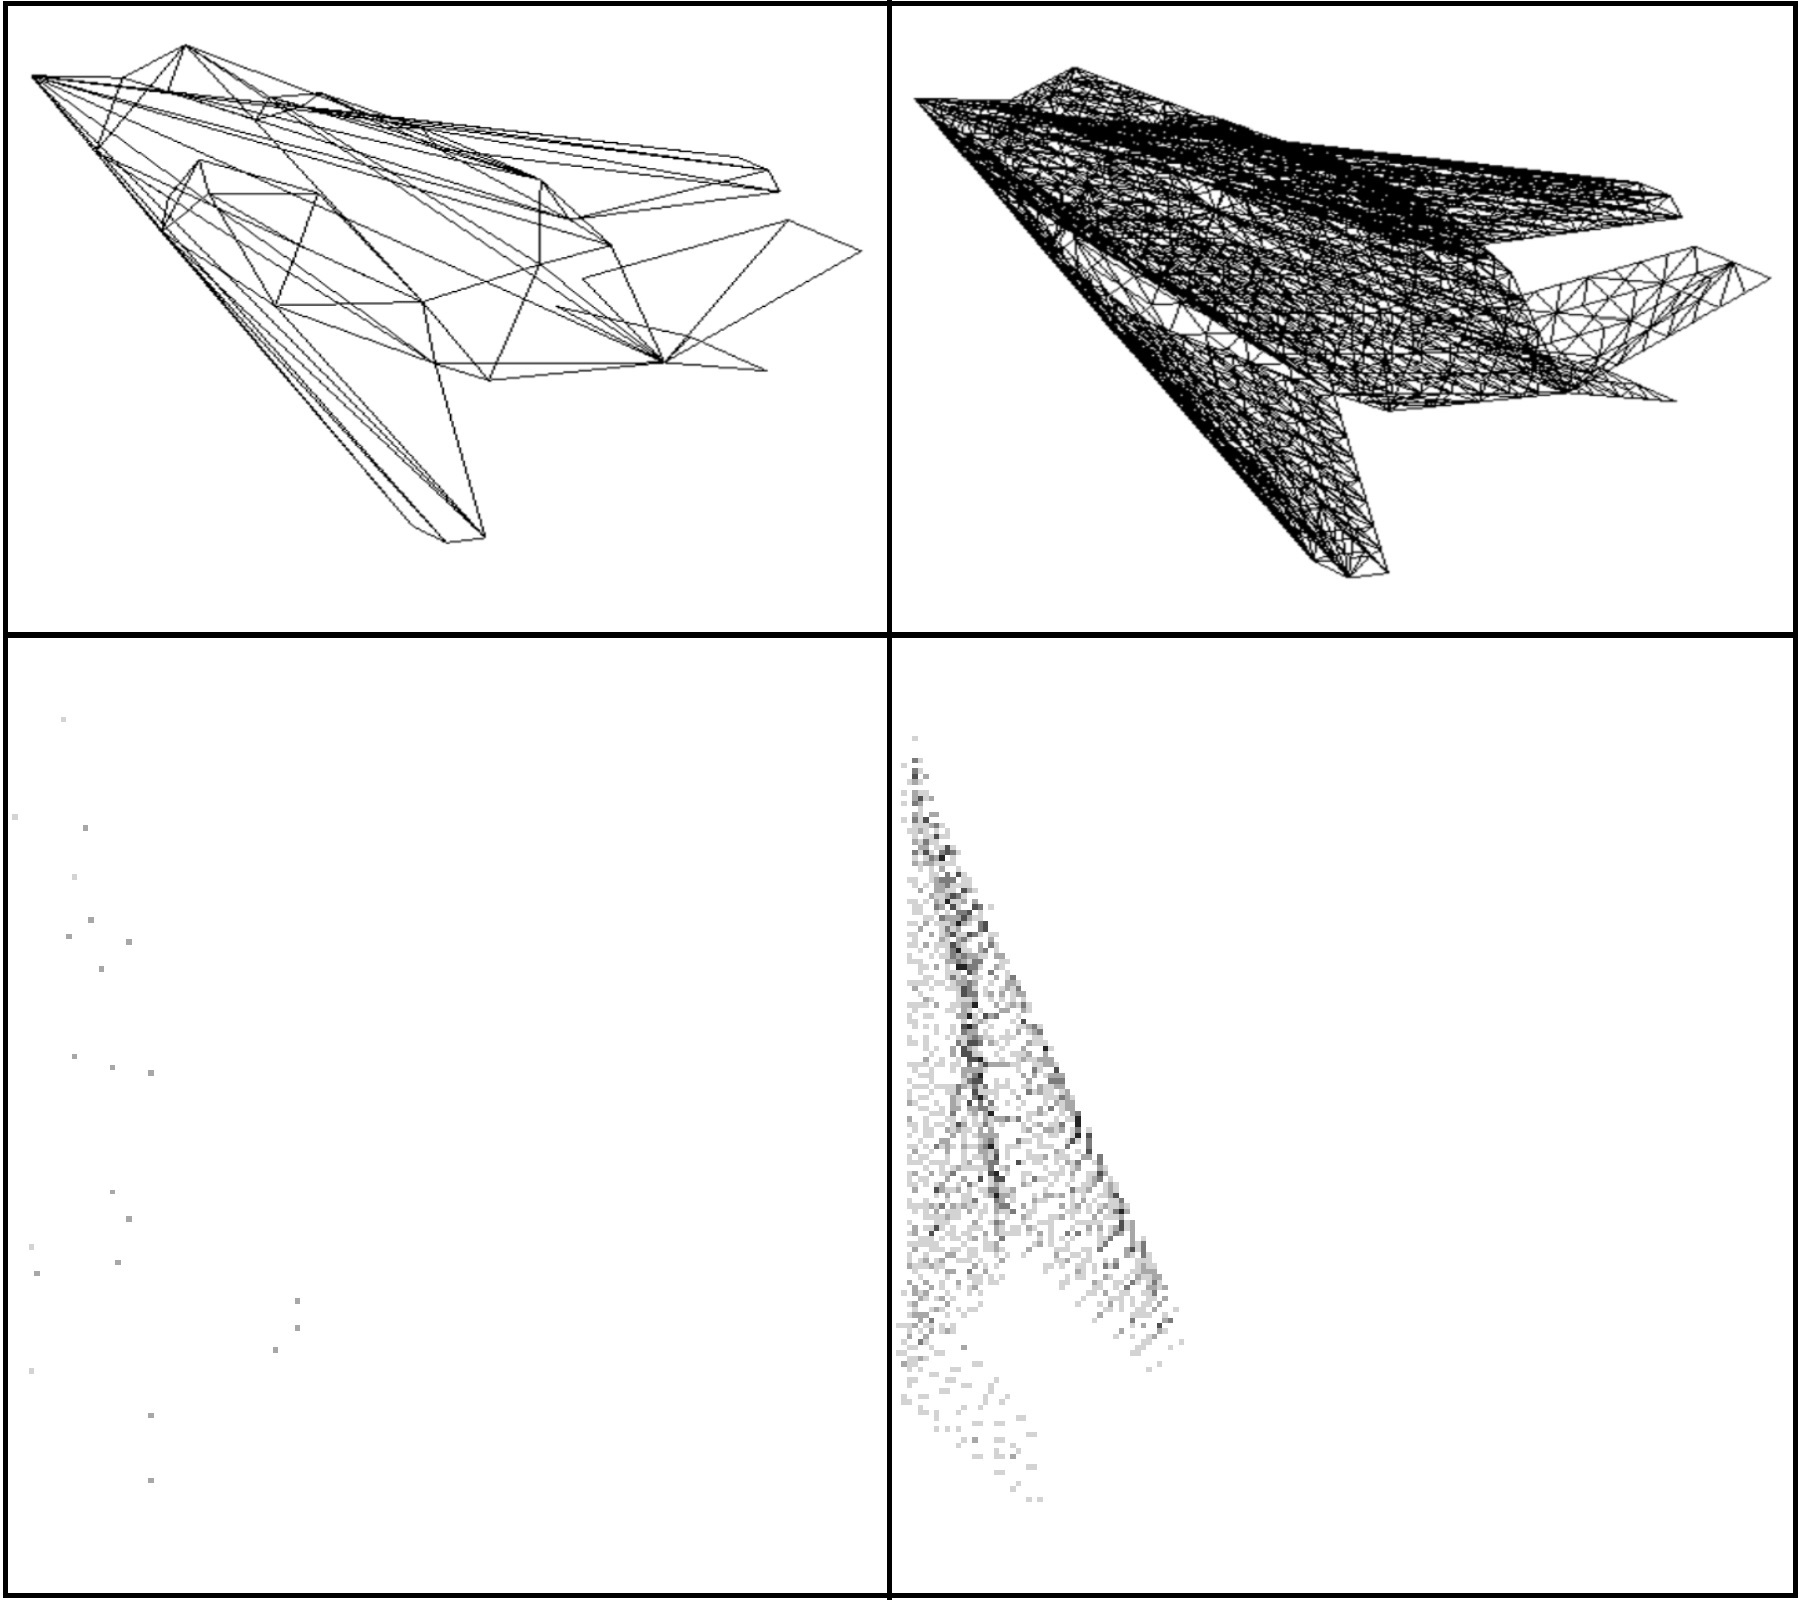
\includegraphics[scale=0.3]{5.JPG}
		\caption{Спиновые изображения одной и той же модели с разной средней длинной ребер}
		\label{ris:5}
	\end{center}
\end{figure}

Решение данной проблемы было представлено в работе \cite{Spin}. Далее предлагается в деталях рассмотреть описание и реализацию алгоритма контроля разрешения трехмерных полигональных моделей.

Для произвольных трехмерных объектов невозможно иметь одинаковое расстояние между всеми вершинами и при этом адекватно описать их форму. Таким образом, длины ребер могут быть измерены с использованием локальных и глобальных статистических данных. Наглядно эти данные удобно рассматривать с помощью гистограммы. Пример такой гистограммы представлен на рис.\ref{ris:mc1}.

\begin{figure}
	\begin{center}
		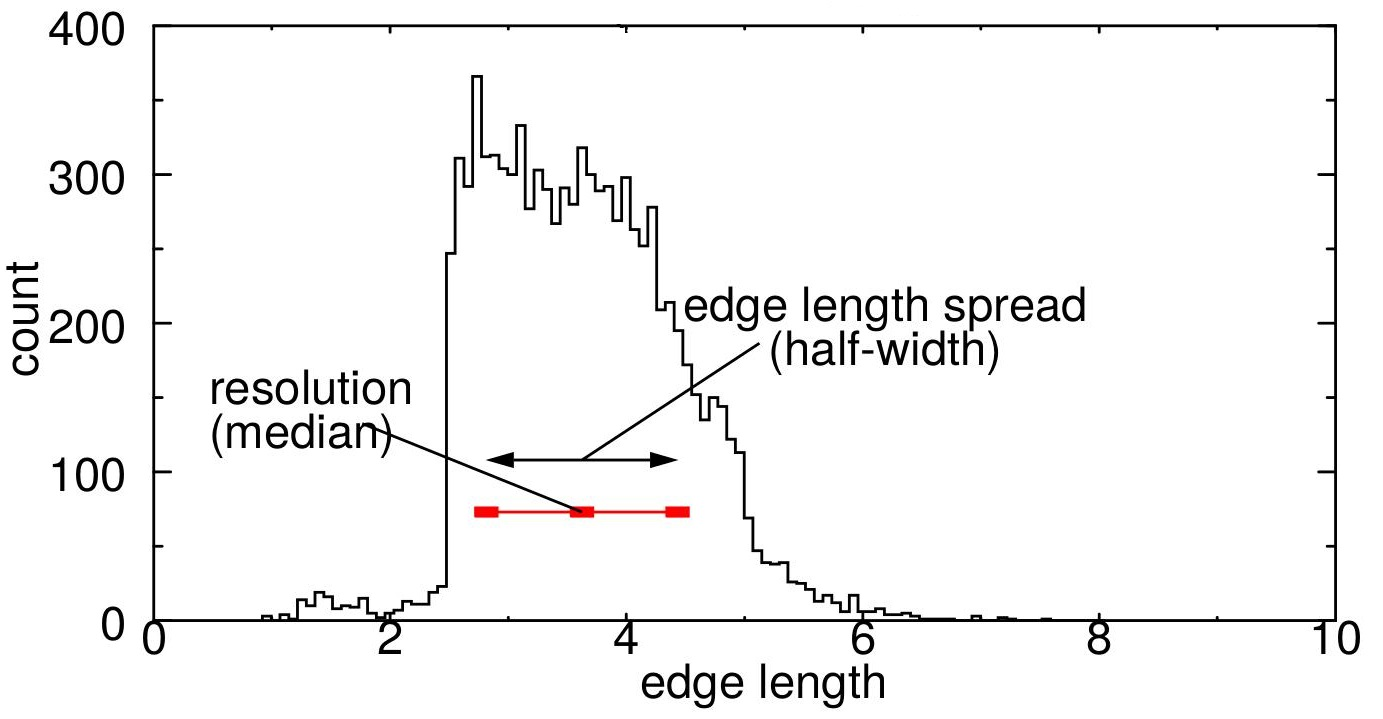
\includegraphics[scale = 0.6]{mc1.JPG}
		\caption{Гистограмма отражающая количество ребер определенной длины в трехмерном объекте}
		\label{ris:mc1}
	\end{center}
\end{figure}

На данной гистограмме по горизонтальной оси представлены длины ребер, а по вертикальной количество ребер определенной длины в объекте. Также по гистограмме можно оценить разрешение объекта и его длину распространения ребра. Определим разрешение объекта как медиану длин всех его ребер, а длину распространения ребра как верхнюю квартиль длин ребер минус нижнюю квартиль длин ребер (то есть, половину ширины). Учитывая эти определения, цель алгоритма - привести исходное разрешение объекта к желаемому путем минимизации длины распространения ребра в гистограмме. Назовем этот процесс нормализацией длины.

Дополнительным ограничением на нормализацию длины ребра является то, что первоначальная форма объекта должна быть сохранена. Предполагается, что первоначальная форма объекта определяется сетью точек и ребер поданной на вход алгоритма. Для получения нужного разрешения, к ребрам модели применяются две операции:

\begin{enumerate}
	\item
	edge-split - убрать длинное ребро;
	\item
	edge-collapse - убрать короткое ребро.
\end{enumerate}

Реализация методов, соответствующих данным операциям приведена в Приложении А.

Во время edge-split ребро разделяют в его средней точке на два ребра. Эта операция не меняет форму объекта. Во время edge-collapse ребро превращается в точку, по этому локально форма поверхности изменяется. В рассматриваемом алгоритме положение результирующей точки после edge-collapse выбирают так, чтобы сохранить форму объекта, но некоторые изменения формы неизбежны, когда ребра приходится удалять. Тем не менее, изменения формы поверхности модели могут быть сведены к минимуму за счет разумного порядка обработки ребер. Более конкретно, ребра упорядочены для работы путем измерения изменения формы объекта, которое является результатом применения операции к каждому ребру. Используя этот порядок, сначала обрабатываются ребра, которые меньше всего изменяют поверхность, тем самым сводя к минимуму изменение формы объекта на каждой итерации. Этот подход позволяет получить объекты, в которых форма поверхности менее отличается от первоначальной при нормализации длины, чем алгоритм, который выбирает ребра случайным образом.

% Для того, чтобы установить баланс между сохранением формы и нормализацией длины ребер в сетке, порядок применения операций к ребрам также зависит от длины ребер к которым пименяется операция. Более конкретно \textbf{вес длины ребра (edge length weight)} вычисляется для каждого ребра; порядок в котором ребра обрабатываются, определяется произведением(?) edge length weight и shape change measure. К примеру, используя данный порядок, для двух ребер с одинаковыми shape change measure длинна которых меньше целевого разрешения, более короткое ребро будет удалено первым.

Предотвратить слишком сильное изменение поверхности модели возможно, путем размещения ограничения на максимально допустимое изменение в формы объекта.
%Каждый раз, когда к какому-либо ребру применяется операция, изменяющая форму объекта, его мера изменения формы добавляется в переменные которые контролируют изменение формы для всех соседних ребер. Если общее изменение формы поверхности больше чем максимально допустимое, ребро снимается с рассмотрения и происходит переход к следующему. Это гарантирует, что, по всей поверхности сетки, изменение формы останется ниже определенной пользователем границы.

Если рассматриваемое ребро укладывается в установленные границы его длины, оно не будет уничтожено. Ограничение на максимальное изменение формы и нахождение длины ребра в некотором допустимом интервале исключает удаление всех ребер. Это является критерием остановки алгоритма. Так как алгоритм направлен на нормализацию длины ребер, сохраняя при этом форму объекта, очевидно, что большинство, но не все, из длин ребер будут находится в установленном допустимом интервале.

Для корректного описания алгоритма в деталях стоит определить понятия ближайших соседей ребер и вершин поверхности объекта. Названия данных сущностей, приведенные в данной работе, соответствуют названиям методов их поиска в реализованном алгоритме.
%!!!названиям методов их поиска в реализованном алгоритме

Пусть EdgeStar(e) соответствует ближайшим соседям ребра $e$, когда к нему применяется операция edge-collapse. EdgeStar(e) содержит все грани, в которых есть как минимум одна из вершин ребра $e$ вместе с ребрами и вершинами, которые составляют данные грани. Определим VertexStar(v) как ближайших соседей вершины $v$ которые созданы после применения к ребру операции edge-collapse. VertexStar(v) содержит все грани, содержащие вершину $v$ вместе с составляющими ее ребрами и вершинами. Иллюстрации EdgeStar(e) и VertexStar(v) приведены на рис.\ref{ris:mc2}.

\begin{figure}
	\begin{center}
		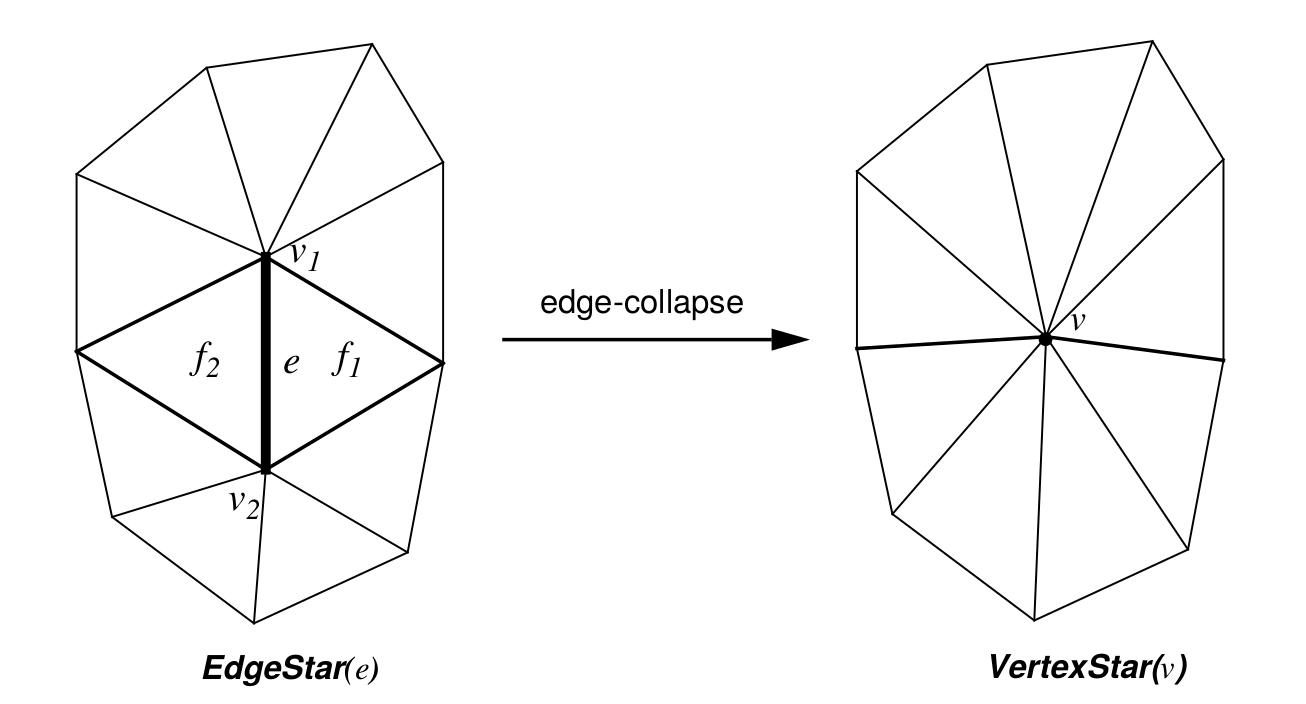
\includegraphics[scale = 0.3]{mc2.JPG}
		\caption{Влияние edge-collapse на его ближайших соседей: ребро $e$ свернуто в вершину $v$, при этом удалены ребро $e$, грани $f_1$ и $f_2$, и вершины $v_1$ и $v_2$}
		\label{ris:mc2}
	\end{center}
\end{figure}

Пусть EdgeDiamond(e) соответствует ближайшим соседям ребра $e$ перед применением к нему операции edge-split. EdgeDiamond(e) содержит грани, примыкающие к ребру $е$. Ребра и вершины, составляющие эти грани также включены в EdgeDiamond(e). Также определим VertexDiamond(v) для вершины $v$ как ее ближайших соседей после применения к ней операции edge-split. VertexDiamond(v) содержит четыре грани которые составлены из вершины $v$ вместе с ребрами и вершинами которые включены в данные грани. Иллюстрации EdgeDiamond(e) и VertexDiamond(v) приведены на рис.\ref{ris:mc3}.

\begin{figure}
	\begin{center}
		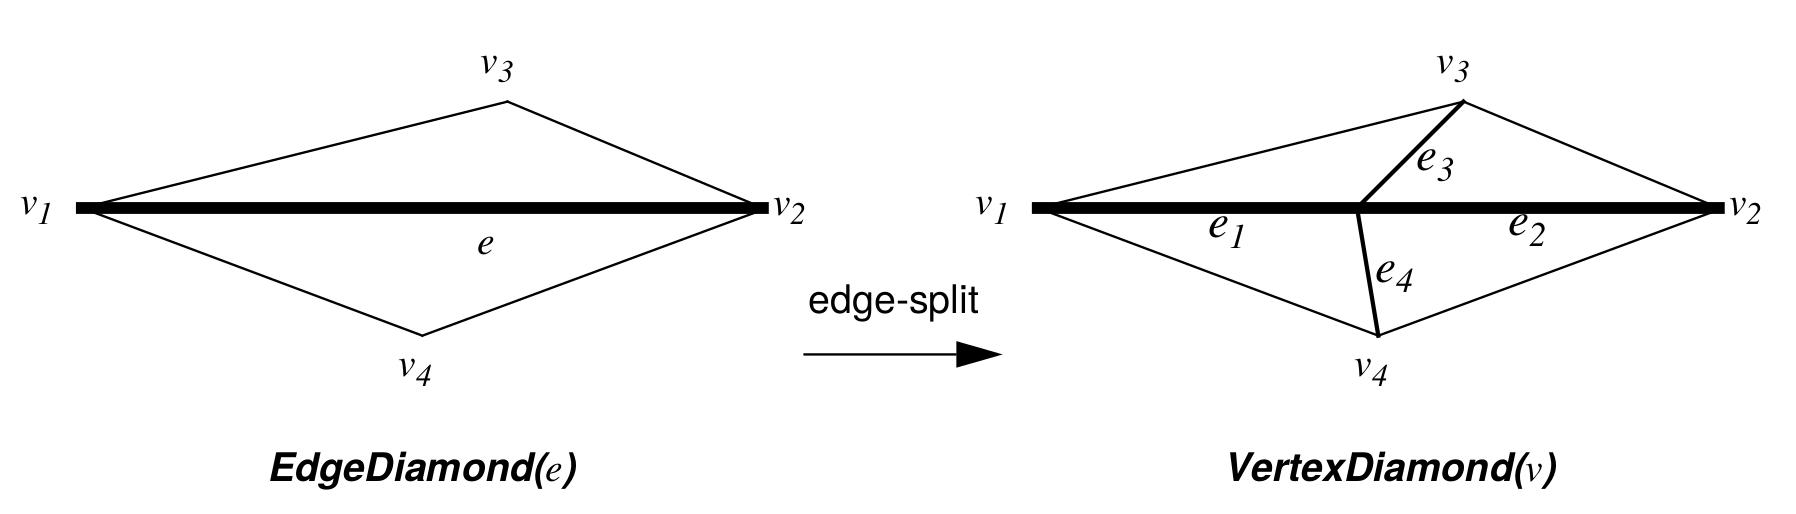
\includegraphics[scale = 0.25]{mc3.JPG}
		\caption{Влияние edge-split на его ближайших соседей: ребро $e$ разбито вершиной $v$, добавлены три новых ребра две новые грани; ближайшие соседи $e$ перед edge-split - EdgeDiamond(e), а ближайшие соседи вершины $v$ после edge-split - VertexDiamond(v)}
		\label{ris:mc3}
	\end{center}
\end{figure}

\subsection{Обзор алгоритма}

Входом в алгоритм служит желаемое разрешение $L_0$ и допустимое отклонение длины ребер $L_D$ от $L_0$ в нормализованном объекте. Тогда верхняя и нижняя границы длин ребер:

\begin{equation}
	L_{MIN} = L_0 - \frac{L_D}{2} \qquad L_{MAX} = L_0 + \frac{L_D}{2}
\end{equation}

Также в алгоритм на вход передается максимально возможное изменение формы поверхности $C_{MAX}$.

В деталях, алгоритм выглядит следующим образом: сначала создается динамическая очередь из ребер объекта. Положение ребра в очереди определено его длиной и мерой изменения формы для данного ребра. Таким образом ребра оказываются упорядочены в соответствии с их длиной по убыванию, а ребра с одинаковой длиной расположены таким образом, чтобы сначала обрабатывались те из них, для которых мера изменения формы поверхности будет меньшей. За тем первое ребро в очереди выталкивается из нее и обрабатывается. Если длина ребра больше $L_{MAX}$, ребро разбивается в его средней точке. Разбиение меняет ближайших соседей ребра добавлением новых ребер, граней и вершины. Если длина ребро меньше чем $L_{MIN}$, оно сворачивается в точку, изменяя своих ближайших соседей путем уничтожения ребра и двух граней вместе с их ребрами. Когда ребро сворачивается, его мера изменения формы добавляется в переменные контролирующие изменение формы поверхности для новых ближайших соседей вершины. После проведения данных операций, ближайшие соседи обработанных ребер для старого случая удаляются из очереди. За тем новые ребра добавляются в очередь если они соответствуют следующим критериям:

\begin{enumerate}
	\item
	длина ребер не входит в требуемый интервал для длины ребер $L_{MAX}$ и $L_{MIN}$;
	\item
	накопление изменения формы (accumulated shape change) для этих ребер не больше чем $C_{MAX}$;
\end{enumerate}

Ребра выталкиваются из очереди и обрабатываются пока очередь не станет пустой.

\subsection{Мера изменения формы}

Мера изменения формы определяется как разница между старой и новой поверхностью до и после обработки ребра. Как уже упоминалось ранее, перед началом работы алгоритма пользователь определяет максимально возможное изменение формы поверхности $C_{MAX}$. Поскольку обработка ребра влияет только на его ближайших соседей, разница между старой и новой формой объекта на одной итерации может быть измерена путем сравнения только окрестности (ближайших соседей) обрабатываемого ребра до и после проведения над ним необходимых операций.

Логично предположить, что форма объекта должна определяться его гранями, поэтому точная мера изменения между старой и новой моделью должна учитывать расстояние между гранями. Определим расстояние между поверхностями $M_1$ и $M_2$ как максимальное расстояние между любой точкой на $M_1$ и ее ближайшей связанной точкой на $M_2$. Поскольку модели представляют собой объединение подмножеств линейных элементов (точки, линии и плоскости), максимальное отличие $M_1$ и $M_2$ заключено между вершиной на $M_1$ и гранью из $M_2$. Отсюда следует что разница между $M_1$ и $M_2$ определяется как максимум Евклидова расстояния между вершиной $v_i$ из $M_1$ и ближайшей к ней точкой, $v_{closest}$, на грани $f_i$ из $M_2$.

\begin{equation}
	d(M_1, M_2) = \max_{v_i \in M_1}(\min_{f_i \in M_2}||v_i - v_{closest}(v_i, f_i)||)
\end{equation}

%!!!

Ближайшая точка на треугольнике к точке в пространстве определена как проекция этой точки на плоскость данного треугольника. Если спроецированная точка лежит внутри треугольника, тогда - это и есть искомая точка. В противном случае точка перпендикулярно проецируется на прямые, на которых лежат стороны треугольника. Если проекция точки расположена между двумя вершинами треугольника, тогда - это искомая точка. В противном случае, искомой точкой является одна из вершин треугольника.

%!!!

Расстояние $d(M_1, M_2)$ не симметрично, поэтому определим показатель различия между двумя поверхностями $D(M_1, M_2)$ как максимум между $d(M_1, M_2)$ и $d(M_2, M_1)$:

\begin{equation}
	D(M_1, M_2) = max(d(M_1, M_2), d(M_2, M_1))
\end{equation}

В представленном алгоритме нормализации длины ребер будем использовать $D(M_1, M_2)$ как меру изменения формы. Очевидно, что мера изменения формы будет равна нулю, когда поверхности совпадают, даже если грани, ребра и вершины не являются точно равными. Использование максимального различия между поверхностями как меры изменения формы дает алгоритму возможность обрабатывать ребра вдоль поверхностных неоднородностей модели, таких как гребни или углы, пока различие между объектами остается малым во время обработки ребер.

% В целом сравнение сеток, вычислением $D(M_1, M_2)$ достаточно затратно в плане вычислений. Однако, как будет показано в следующем параграфе, вычисление меры изменения формы между сетками до и после обработки ребра является осуществимым с вычислительной точки зрения когда изменения в сетке ограничены ближайшими соседями ребра в сетке.

\subsection{Базовые операции алгоритма}

В данном подразделе подробно рассматриваются операции edge-collapse и edge-star, и некоторые особенности их реализации.

Первой рассмотрим операцию edge-collapse. Как показано на рис.\ref{ris:mc2} цель данной процедуры - сжать ребро в точку посредством этого удаляя ребро и две смежные с ним грани. Операция edge-collapse может быть представлена через локальные операции, которые удаляют задействованные ребра и вершины с поверхности модели в наборе данных, а за тем добавляют новые ребра в очередь.

Важной переменной является позиция новой вершины, которая является результатом edsge-collapse. Позиции остальных вершин в EdgeStar(e) остаются неизменными в течении edge-collapse. Простым решением является поместить результирующую точку в центр сворачиваемого ребра. Однако, как показано на рис.\ref{ris:mc5} (слева), размещение новой вершины на поверхности сети объекта может вызвать чрезмерное изменение формы (усадку или расширение) в районах с высокой кривизной поверхности.

\begin{figure}
	\begin{center}
		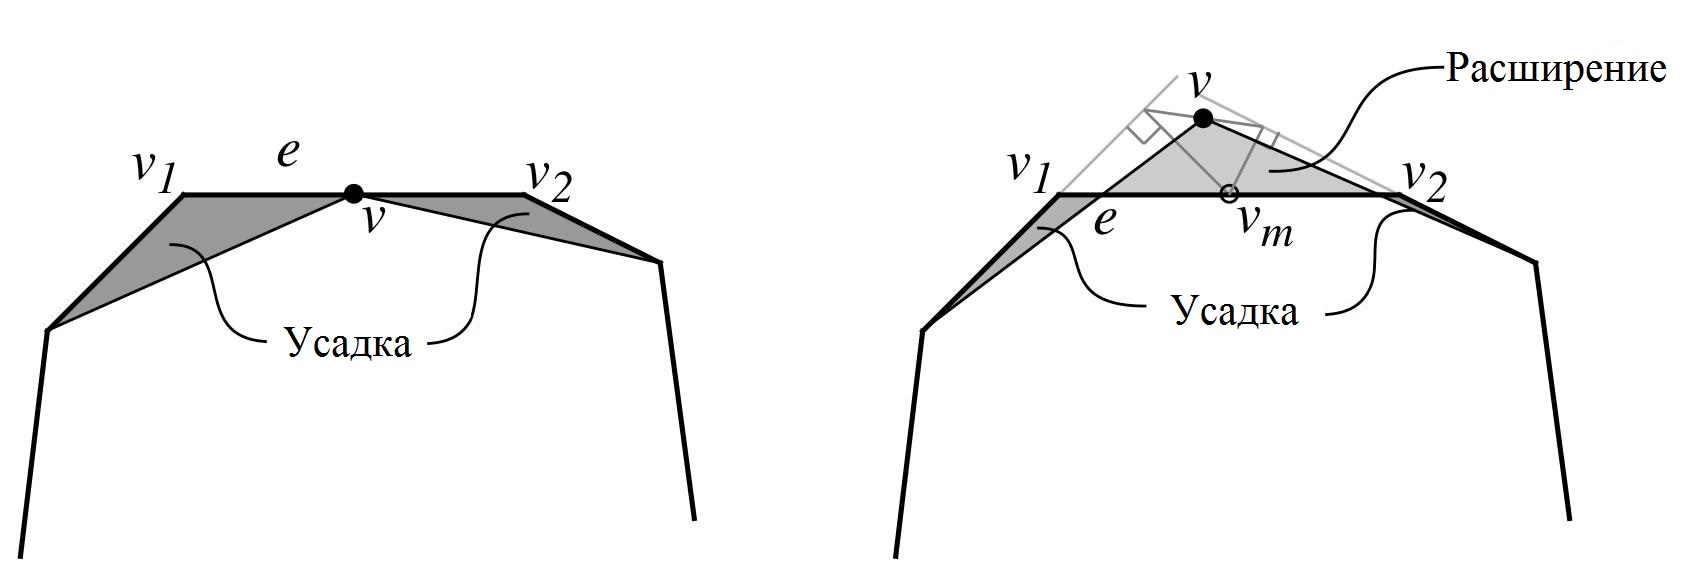
\includegraphics[scale = 0.47]{mc5.JPG}
		\caption{Расположение результирующей точки после операции edge-collapse}
		\label{ris:mc5}
	\end{center}
\end{figure}

Таким образом в большинстве случаев стоит поместить вершину, которая получена после edge-collapse вне прямой, на которой лежит удаляемое ребро. В частности, за позицию новой вершины $v$ следует принять среднее проекций середины сворачиваемого ребра $v_m$ на $N$ плоскостей которым принадлежат грани из EdgeStar(e).

\begin{equation}
	v = v_m - \frac{1}{N} \sum\limits_{i = 1}^N (n_i v_m + d_i)n_i \qquad v_m = \frac{v_1 + v_2}{2}
\end{equation}

Грани из EdgeStar(e) в этом случае определяются нормалями плоскостей на которых лежат эти грани $n_i$ и их смещением $d_i$ относительно центра сворачиваемого ребра $v_m$. На рис.\ref{ris:mc5} (справа) представлен пример расположения новой вершины после применения операции edge-collapse на основе проецирования середины сворачиваемого ребра на соседние плоскости. Таким образом усадка сети объекта предотвращается путем распределения изменения формы поверхности выше и ниже уничтоженного ребра.

Мера изменения формы для ребра, которое мы собираемся свернуть в точку может быть вычислена, используя EdgeStar(e) и VertexStar(v). После edge-collapse вершины вдоль границы VertexStar(v) те же что и вершины на границе EdgeStar(e). Таким образом, в соответствии с рис.\ref{ris:mc2}, мера изменения формы может быть вычислена как максимум расстояния между $v$ и ее ближайшей точкой на гранях EdgeStar(e), $v_1$ и ее ближайшей точкой на гранях VertexStar(v), или $v_2$ и ее ближайшей точкой на гранях VertexStar(v).

% \begin{center}
% 	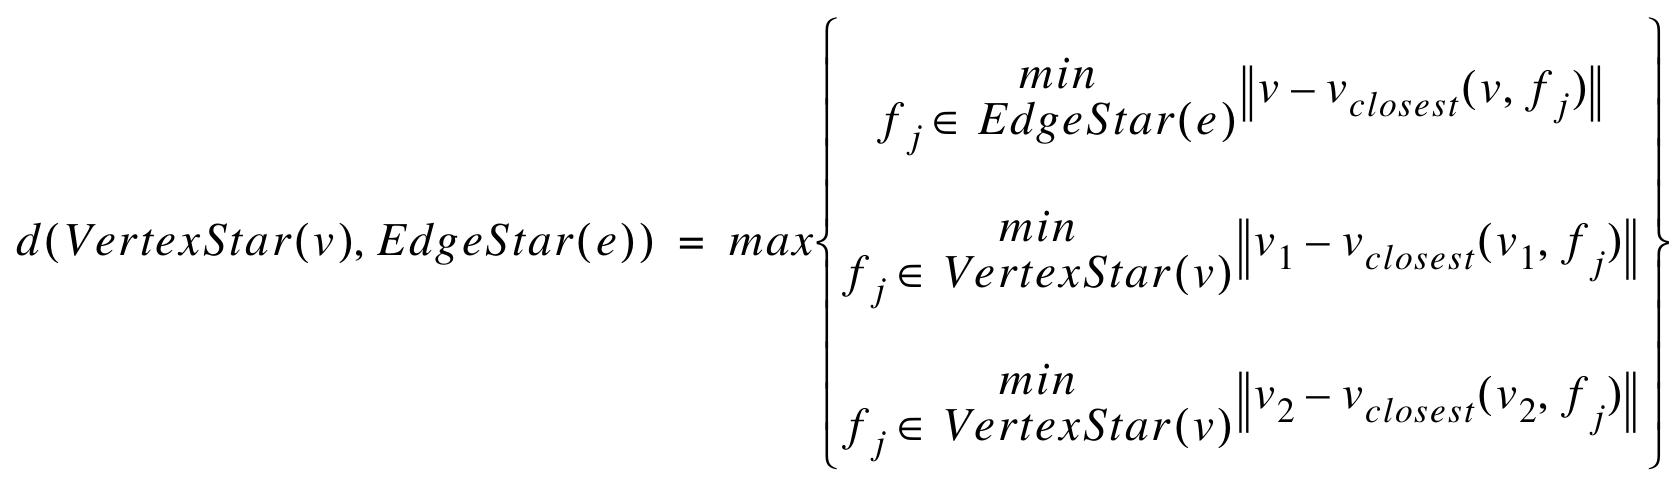
\includegraphics[scale = 0.29]{mc6.JPG}
% \end{center}

Теперь рассмотрим операцию edge-split. Она используется чтобы убрать слишком длинные ребра. Как показано на рис.\ref{ris:mc3}, edge-split делит ребро вершиной и производит новые ребра, две новые грани и новую вершину. Позиция новой вершины выбирается в середине разделяемого ребра. Так как поверхность до и после edge-split не изменяется, значит мера изменения формы для этой операции всегда равна нулю и не рассматривается в процессе работы алгоритма. Операция edge-split может быть реализована через локальные изменения поверхности, которые добавляют новые ребра и вершину в очередь и за удаляют разделяемое ребро из очереди.

\subsection{Накопление изменения формы}

Определим накопление изменения формы как некоторое значение, которое соответствует изменению формы всей модели в процессе нормализации длины ее ребер. Как было рассмотрено ранее, каждый раз после удаления ребра, форма объекта немного меняется. Мера изменения формы в нашем случае - это максимальное расстояние между поверхностями до и после сворачивания ребра для его ближайших соседей.
%Ограничим величину накопления изменения формы, к которой приводит нормализация, путем хранения изменения формы сетки для всей модели.
Первоначально у каждого ребра нулевая мера изменения формы, а у модели нулевое накопление изменения формы. Когда ребро $e$ свернуто, его мера изменения формы вычисляется и добавляется накопление изменения формы. Отслеживая худший случай изменения формы для каждого ребра, мы можем ограничить глобальный максимум изменения формы объекта. Другими словами, ребра, при сворачивании которых накопление изменения формы может превысить максимально возможное изменение формы поверхности $C_{MAX}$, следует удалить из очереди, несмотря на то, что они могут не входить в целевой интервал для длины ребер.

\newpage

\section{Сверточные нейронные сети}

\subsection{Общие представления}

Компьютерные методы, имитирующие человеческое зрение, сегодня используются для решения многих задач – от определения лиц на Facebook и автопилотируемых Google-мобилей до суперсовременных алгоритмов диагностики заболеваний. Однако на поверку имитация работы человеческих органов зрения оказывается задачей не из легких. Там, где мы автоматически распознаем линии, контуры и объекты, компьютер видит всего лишь огромные числовые матрицы.

Для решения задачи определения более сложных признаков из сырых массивов пикселов предлагается использовать отдельный тип нейронных сетей, называемых сверточными.

Свёрточная нейронная сеть (convolutional neural network, CNN, LeNet) была представлена в 1998 году французским исследователем Яном Лекуном (Yann LeCun) \cite{LeCun}, как развитие модели неокогнитрон \cite{Fukushima}. Архитектура данного типа нейронных сетей схожа с некоторыми особенностями зрительной коры, в которой имеются простые клетки, реагирующие на прямые линии под разными углами, и сложные клетки, реакция которых связана с активацией определённого набора простых клеток.

Таким образом, идея свёрточных нейронных сетей заключается в чередовании свёрточных слоев (англ. convolution layers) и субдискретизирующих слоев (англ. subsampling/pooling layers). Для обучения используются градиентные методы, чаще всего метод обратного распространения ошибки.

Название архитектура сети получила из-за наличия операции свёртки \cite{Borisov1}, суть которой в том, что каждый фрагмент изображения умножается на матрицу (ядро) свёртки поэлементно, а результат суммируется и записывается в аналогичную позицию выходного изображения.

\begin{equation}
	(f * g)[m, n] = \sum_{k,l}{f[m - k, n - l] \cdot g[k, l]}
\end{equation}

Здесь f - исходная матрица изображения, g - ядро (матрица) свёртки.

Теперь выделим некоторые преимущества и недостатки, данного типа нейронных сетей.

Преимущества:
\begin{enumerate}
	\item
	По сравнению с полносвязной нейронной сетью — в сверточной нейронной сети требуется гораздо меньшее количество настраиваемых весов, так как одно ядро весов используется целиком для всего изображения, вместо того, чтобы делать для каждого пикселя входного изображения свои персональные весовые коэффициенты. Это подталкивает нейросеть при обучении к обобщению демонстрируемой информации, а не попиксельному запоминанию каждой показанной картинки в мириадах весовых коэффициентов, как это делает перцептрон.
	\item
	Удобное распараллеливание вычислений, а, следовательно, возможность реализации алгоритмов работы и обучения сети на графических процессорах.
	\item
	Относительная устойчивость к повороту и сдвигу распознаваемого изображения.
	\item
	Обучение при помощи классического метода обратного распространения ошибки.
\end{enumerate}

Недостатки:
\begin{enumerate}
	\item
	Архитектура свёрточной нейронной сети по большей части пригодна только для распознавания изображений.
	\item
	Слишком много варьируемых параметров сети. Существует несколько выверенных и прекрасно работающих конфигураций сетей, но нет правил, по которым нужно делать выбор для новой задачи.
\end{enumerate}

\subsection{Архитектура сверточной нейронной сети}

Модель свёрточной сети рис.\ref{ris:6}, состоит из трёх типов слоёв: свёрточные \\ (convolutional) слои, субдискретизирующие (subsampling/pooling) слои и слои "обычной" полносвязной нейронной сети (fully-connected layer).

\begin{figure}[h]
	\begin{center}
		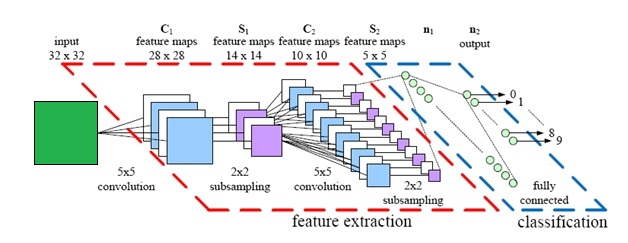
\includegraphics[scale=0.99] {6.JPG}
		\caption{Общая схема свёрточной нейронной сети}
		\label{ris:6}
	\end{center}
\end{figure}

Первые два типа слоёв (convolutional, subsampling/pooling), чередуясь между собой, формируют входной вектор признаков для многослойного перцептрона (fully connected MLP).
% Сеть можно обучать с помощью градиентных методов \cite{Borisov2}.

Далее рассмотрим подробнее каждый из типов слоев сверточной нейронной сети.

\subsubsection{Свёрточный слой}

Свёрточный слой ( англ. Convolutional layer ) является основным строительным блоком сверточной нейронной сети. Параметры слоя состоят из набора фильтров для обучения (или ядер свертки), которые имеют небольшое рецептивное поле, но простираются на всю глубину входной матрицы. В течение прямого прохода каждый фильтр осуществляет свертку по ширине и высоте матрицы на входе, вычисляя скалярное произведение данных фильтра и входа, и формируя двумерную карту активации этого фильтра.

Размерность матрицы на выходе сверточного слоя контролируют три гиперпараметра: глубина(depth), шаг(stride) и нулевое дополнение(zero-padding).

\begin{enumerate}
	\item
	Глубина контролирует количество нейронов слоя, которые соединяются с одной и той же областью изображения на входе. Другими словами, это количество ядер свертки в данном слое.
	\item
	Шаг контроллирует перемещение ядра свертки по входной матрице. Например, если шаг равен 1, то ядро свертки каждый раз перемещается на один пиксель.
	\item
	Иногда удобно дополнять вход нулями по краям входной матрицы. Размер этого нулевого дополнения является третьим гиперпараметром. Нулевое дополнение позволяет контролировать пространственный размер выходных матриц.
\end{enumerate}

Пространственный размер выходной матрицы $W_2$ может исчисляться как функция от размера входной матрицы $W_1$, размера рецептивного поля нейронов сверточного слоя $F$, шага, с которым они применяются $S$, и величины нулевого дополнения $P$, применяемой на краях \cite{Stanford}.

\begin{equation}
	W_2 = \frac{W_1 - F + 2P}{S} + 1
\end{equation}

Если это число не является целым, то шаги установлено неправильно, и нейроны не могут быть размещены вдоль входной матрицы симметричным образом. В общем случае, установление нулевого дополнения в $P = (F - 1) / 2$, когда шагом является $S = 1$, обеспечивает, чтобы входной и выходной объемы имели одинаковый пространственный размер.

Следует также отметить, что глубина выходной матрицы равна количеству примененных ядер свертки(фильтров).

\subsubsection{Субдискретизирующий слой}

При реализации архитектуры сверточных нейронных сетей, между последовательно идущими сверточными слоями обычно помещают субдискретизирующие слои. Слои этого типа выполняют уменьшение размера входной карты признаков. Это можно делать разными способами, в данном случае рассматривается метод выбора максимального элемента (max-pooling) - вся карта признаков разделяется на ячейки $[2 \times 2]$ элемента, из которых выбираются максимальные по значению рис.\ref{ris:7}.

\begin{figure}[h]
	\begin{center}
		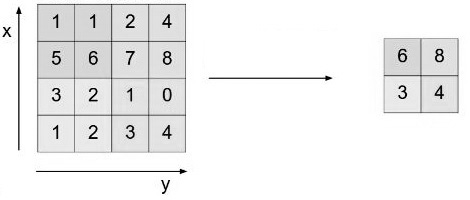
\includegraphics[scale=0.7] {7.JPG}
		\caption{Пример выбора максимальных элементов из матрицы 4х4 при действии на нее pooling слоем размерности 2х2}
		\label{ris:7}
	\end{center}
\end{figure}

Субдискретизирующий слой формирует размер выходной матрицы $W_2$ как функцию от размера входной матрицы $W_1$, рецептивного поля $F$ и шага $S$ cубдискретизирующего слоя\cite{Stanford}:

\begin{equation}
	W_2 = \frac{W_1 - F}{S} + 1
\end{equation}

В данном случае глубина выходной матрицы соответствует глубине входной матрицы.

\subsubsection{Слой полносвязной нейронной сети}

Нейроны в полносвязной нейронной сети соединены со всеми картами активаций в предыдущем слое, как в обычных нейронных сетях. На выходе эта нейронная сеть выдает вектор признаков в котором каждый элемент соответствует одному из распознаваемых классов. Чем больше значение одного из элементов этого вектора при работе сети, тем больше, проверяемое изображение соответствует тому или иному классу.

\newpage

\subsection{Обучение сверточных нейронных сетей}

В данном подразделе рассматривается общий принцип обучения сверточной нейронной сети. Первоначально значения весов сверточного слоя инициализированы случайным образом. Корректировку их значений в данной работе предлагается провести с помощью метода обратного распространения ошибки\cite{LeCunBackProb}. Данный метод предполагает корректировать веса с помощью обучающего набора изображений у каждого из которых есть ярлык, говорящий о принадлежности данного изображения определенному классу.

Метод обратного распространения ошибки можно разделить на четыре этапа: прямое распространение, функцию потери, обратное распространение и обновление веса. Во время прямого распространения, тренировочное изображение пропускается через всю сеть и регистрируется полученный результат. Сравнение полученного и желаемого результатов - есть качество распознавания. Для получения возможности такого сравнения определим функцию потери обучающей пары. В данной работе предлагается использовать функцию среднеквадратической ошибки:

\begin{equation}
    L(W) = (\sum\limits_{p = 1}^{N} \frac{1}{2}(D_p - O(I_p, W))^2) / N
\end{equation}
,где $L(W)$ — это функция ошибки для всей обучающей выборки, $p$ - номер обучающей пары, $N$ - количество обучающих пар, $D_p$ — желаемый выход сети, $O(I_p,W)$ — выход сети, зависящий от $p$-го входа и весовых коэффициентов $W$. Задача обучения так настроить веса $W$, чтобы они для любой обучающей пары $(I_p,D_p$) давали минимальную ошибку $L$. Для этого сначала нужно выяснить, какие веса самым непосредственным образом способствовали ошибкам сети, а затем скорректировать их так, чтобы снизить потерю.

Значение производной функции ошибки по одному из весовых коэффициентов($\frac{dL}{dW}$) определяет влияние этого веса на ошибки сети. При обратном распространении данная производная вычисляется для весов каждого слоя после чего происходит обновление весов на рассматриваемом слое. Формула по которой происходит корректировка каждого фильтрового веса приведена ниже:

\begin{equation}
    w = w_i - \eta\frac{dL(W_i)}{dW}
\end{equation}
,где $w_i$ - начальное значение регулируемого веса, $L(W_i)$ - функция ошибки, $\eta$ - скорость обучения.

В данной формуле параметр, который отвечает за скорость обучения, выбирается программистом. По своей сути он определяет шаг, с которым будет корректироваться вес. Он должен быть выбран таким образом, чтобы, с одной стороны, корректировка фильтровых весов была достаточно точной без слишком больших скачков, а с другой - позволила бы достичь минимума функции ошибок к окончанию обучения.

Процесс прямого распространения, функцию потери, обратное распространение и обновление весов обычно называют одним периодом дискретизации (или epoch — эпохой). Программа будет повторять этот процесс фиксированное количество периодов для каждого тренировочного изображения. После того, как обновление параметров завершится на последнем тренировочном образце, сеть в теории должна быть достаточно хорошо обучена и веса слоёв настроены правильно.

\newpage

\section{Реализация системы классификации трехмерных моделей}

В данном разделе представлена реализация системы классификации трехмерных объектов и результаты ее тестирования.

\subsection{Подготовка данных для обучения сверточной нейронной сети}

Для реализации подобной системы было решено использовать модели, представленные в базе трехмерных моделей университета Princeton, а именно 180 объектов трех различных классов: "Самолет" (airplane aircraft), "Мебель" (furniture) и "Человек" (human). Для контроля разрешения трехмерных моделей, алгоритм, представленный в главе \ref{sect2}, был реализован в виде программы на языке C. При подборе оптимального разрешения моделей стоит отметить, что чрезмерное уменьшение разрешения не только заметно увеличивает время формирования базы данных, но и не ведет к каким-либо преимуществам при обучении сверточной нейронной сети. Это продиктовано тем, что после формирования глобальных дескрипторов в виде интегральных спиновых изображений, значения в "корзинах" дескриптора должны находиться в некотором интервале в зависимости от архитектуры сверточной нейронной сети.

 После подбора оптимального разрешения моделей и формирования окончательной базы данных трехмерных объектов, для каждого из них были получены глобальные дескрипторы в виде интегральных спиновых изображений методом, описанным в работе \cite{Chernikoff}. В результате тестирования систем классификации было установлено, что размер спинового изображения должен быть равен размеру изображений, передаваемых на вход сверточной нейронной сети, а размер корзин должен обеспечивать тот факт, что каждая из корзин будет включена в спиновое изображение (не выйдет за его границы). Также очевидно, что слишком большой размер корзин не обеспечит отражения отличительных признаков каждого класса на дескрипторе. Примеры дескрипторов, использованных для обучения, вы можете видеть на рис.\ref{ris:8}.

 \begin{figure}[h]
 	\begin{center}
 		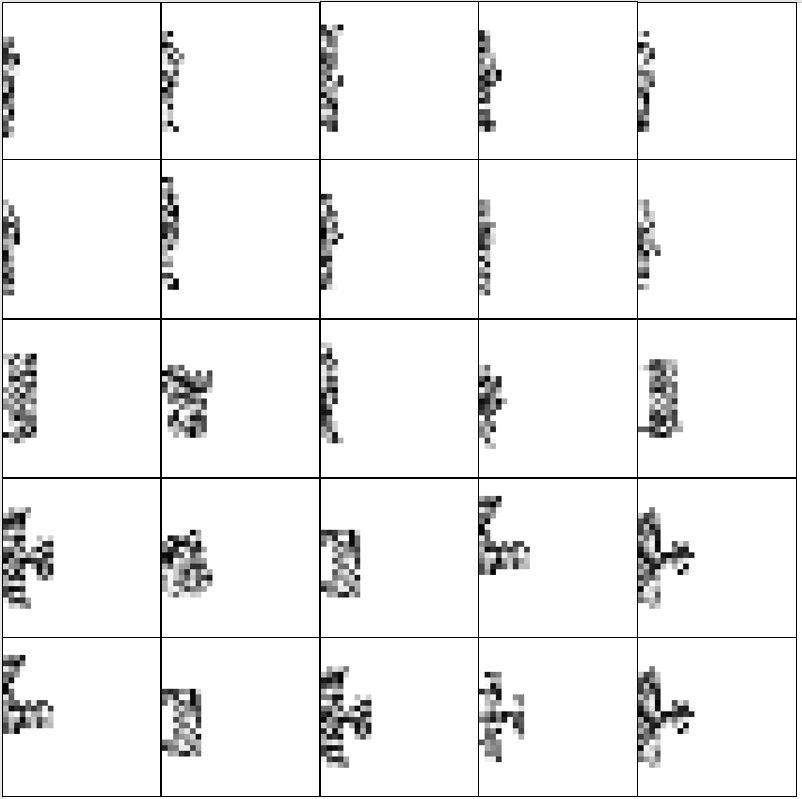
\includegraphics[scale=0.75] {8.JPG}
 		\caption{Примеры глобальных дескрипторов, использованных для обучения сверточных нейронных сетей}
 		\label{ris:8}
 	\end{center}
 \end{figure}

После формирования набора дескрипторов для всех моделей базы данных, происходит этап обучения сверточной нейронной сети. Далее предлагается сравнить результаты обучения сверточных нейронных сетей для двух различных архитектур. В первом случае, за основу архитектуры была принята модель сети, предназначенная для распознавания цветных изображений размерности $[32 \times 32 \times 3]$ - CIFAR-10. Во втором случае сеть строилась на основе архитектуры, предназначенной для классификации рукописных символов из базы изображений MNIST. Реализация данных сверточных нейронных сетей осуществлялась при помощи пакета MatConvNet для Matlab.

 \subsection{Реализация архитектуры на основе сети для цветных изображений}\label{ssec4.2}

Рассмотрим подробнее систему классификации трехмерных объектов в случае, когда за основу архитектуры сверточной нейронной сети была принята сеть, реализующая распознавание десяти классов изображений из базы CIFAR-10. На рис.\ref{ris:9} представлена архитектура данной нейронной сети, адаптированная для классификации трех классов дескрипторов.

\begin{figure}[h]
   \begin{center}
       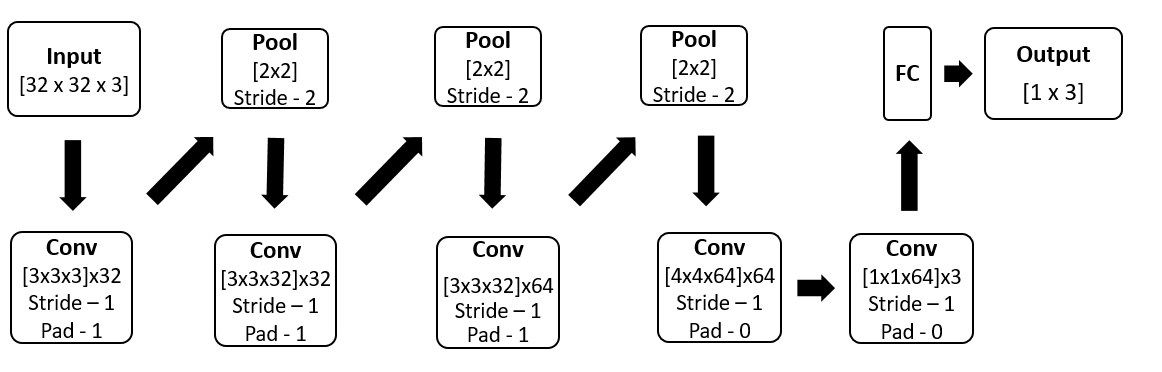
\includegraphics[scale=0.7] {9.JPG}
       \caption{Архитектура сверточной нейронной сети, принимающей на вход объекты размерности $[32 \times 32 \times 3]$}
       \label{ris:9}
   \end{center}
\end{figure}

Прежде всего, стоит отметить, что так как данная нейронная сеть предназначена для распознавания цветных изображений, на вход ей должны передаваться объекты соответствующей размерности $[32 \times 32 \times 3]$. Глобальные дескрипторы поверхности в случае рассматриваемой системы классификации имеют вид двумерных матриц. При подготовке данных значения дескрипторов передаваемые на вход сверточной нейронной сети дублировались для всех трех измерений. Таким образом имитировались цветные изображения из базы данных CIFAR-10. В перспективе возможно использование глобальных дескрипторов поверхности в виде интегральных спиновых изображений с учетом полярного угла как описано в работе \cite{Chernikoff}. Такие спиновые изображения имеют вид трехмерных массивов данных, что делает возможным более корректное использование архитектур сверточных нейронных сетей данного типа.

На рис.\ref{ris:9} можно видеть, что данная архитектура использует пять сверточных слоев и три слоя объединения. В первых двух сверточных слоях(Conv) использовано 32 ядра свертки, на втором и третьем - 64 и на последнем три. Основные гиперпараметры - такие как шаг(Stride) и отступ(Pad) выбирались исключительно методом подбора в зависимости от результатов обучения. На последнем слое сверточной нейронной сети расположена полносвязная нейронная сеть(FC) результатом работы которой является вектор признаков в котором каждый элемент соответствует одному из распознаваемых классов. В Приложении Б представлен программный код реализации данной архитектуры.

Теперь рассмотрим результат обучения данной нейронной сети. На рис.\ref{ris:10} представлен график изменения значений функции ошибки для данной реализации системы. По оси абсцисс данного графика отражены номера эпох обучения, а по оси ординат - значение среднеквадратичной ошибки для каждой эпохи.

\begin{figure}[h]
   \begin{center}
       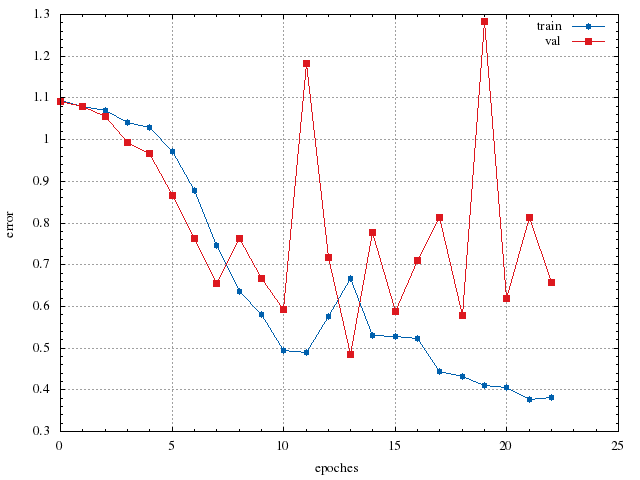
\includegraphics[scale=0.6] {10.JPG}
       \caption{График изменения значений функции ошибки сверточной нейронной сети, принимающей на вход объекты размерности $[32 \times 32 \times 3]$}
       \label{ris:10}
   \end{center}
\end{figure}

Во время обучения сети, обучающая выборка делится на тренировочную(train) и проверочную(validation). После обновления фильтровых коэффициентов для тренировочной выборки, сеть тестируется проверочной выборкой чтобы оценить реальный результат обучения. На графике видно, что значение ошибки для проверочной выборки после некоторого момента перестает снижаться. Это говорит о том, что после этого сеть не продолжает реальный процесс обучения, а лишь затачивается под распознавание тренировочных изображений.

\subsection{Реализация архитектуры на основе сети для рукописных символов}\label{ssec4.3}

В подразделе \ref{ssec4.2} видно, что представленная архитектура не показала хороших результатов, однако сам факт снижения ошибки говорит о том, что сеть способна выделять признаки у глобальных дескрипторов поверхности.

После некоторого количества экспериментов было решено упростить архитектуру сети и искусственно расширить обучающий набор данных в четыре раза путем поворота изображений на 180 градусов и их инвертирования.

За основу архитектуры сверточной нейронной сети была принята модель сети, предназначенная для распознавания рукописных символов из базы изображений MNIST. Размер изображений, передаваемых на вход сети, составляет $28 \times 28$ пикселей. На рис.\ref{ris:11} вы можете видеть рассматриваемую архитектуру, а в Приложении В представлен реализующий ее программный код.

\begin{figure}[h]
   \begin{center}
       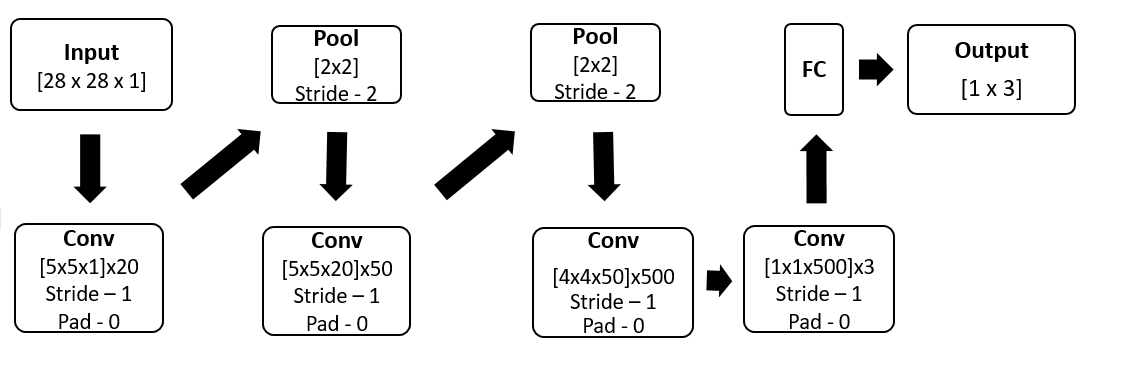
\includegraphics[scale=0.6] {11.JPG}
       \caption{Архитектура сверточной нейронной сети, принимающей на вход объекты размерности $[28 \times 28]$}
       \label{ris:11}
   \end{center}
\end{figure}

При рассмотрении данной архитектуры можно видеть, что данная архитектура использует только четыре сверточных и два слоя объединения. Также значительно увеличено количество ядер свертки на некоторых слоях.

Также стоит отметить, что при подготовке данных из-за уменьшения размера спиновых изображений, передаваемых на вход сверточной нейронной сети, размеры "корзин" спиновых изображений были увеличены по сравнению с реализацией системы классификации, представленной в подразделе \ref{ssec4.2}. В остальном процесс подготовки данных существенно не изменялся.

На рис.\ref{ris:12} представлен график изменения значений функции ошибки для данной реализации системы.

\begin{figure}[h]
   \begin{center}
       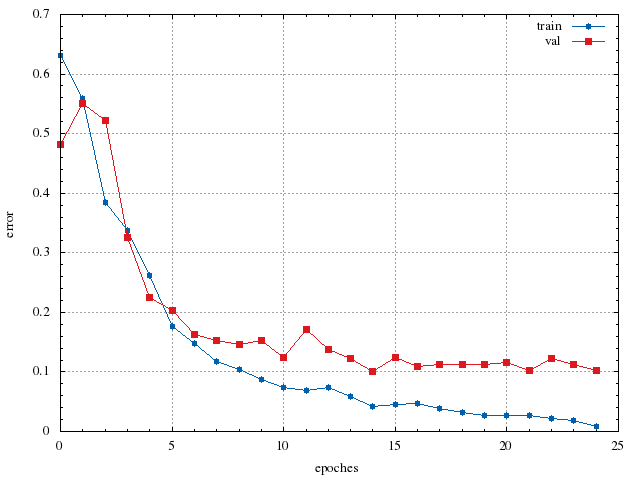
\includegraphics[scale=0.6] {12.JPG}
       \caption{График изменения значений функции ошибки сверточной нейронной сети, принимающей на вход объекты размерности $[28 \times 28]$}
       \label{ris:12}
   \end{center}
\end{figure}

Уже на этапе обучения сети видно, что значение функции ошибки для данной реализации системы снижается для каждой эпохи анализа как для тренировочной, так и для проверочной выборок. Это свидетельствует о том, что сеть выделяет признаки из глобальных дескрипторов, а не просто «запоминает» тренировочные изображения.

\subsection{Анализ результатов работы системы}

Оценим результаты проведенных тестов для систем классификации трехмерных объектов с архитектурами сверточных нейронных сетей, представленных в подразделах \ref{ssec4.2} и \ref{ssec4.3}. На рис.\ref{ris:13} представлена диаграмма, отражающая результат распознавания для 20 случайных моделей трех классов, не входящих в обучающую выборку. В части диаграммы "Реализация системы №1" представлены результаты классификации моделей с использованием архитектуры сверточной нейронной сети, представленной в подразделе \ref{ssec4.2}. Соответственно результат распознавания для архитектуры, представленной в подразделе \ref{ssec4.3} представлен в части диаграммы "Реализация системы №2".

\begin{figure}[h]
   \begin{center}
       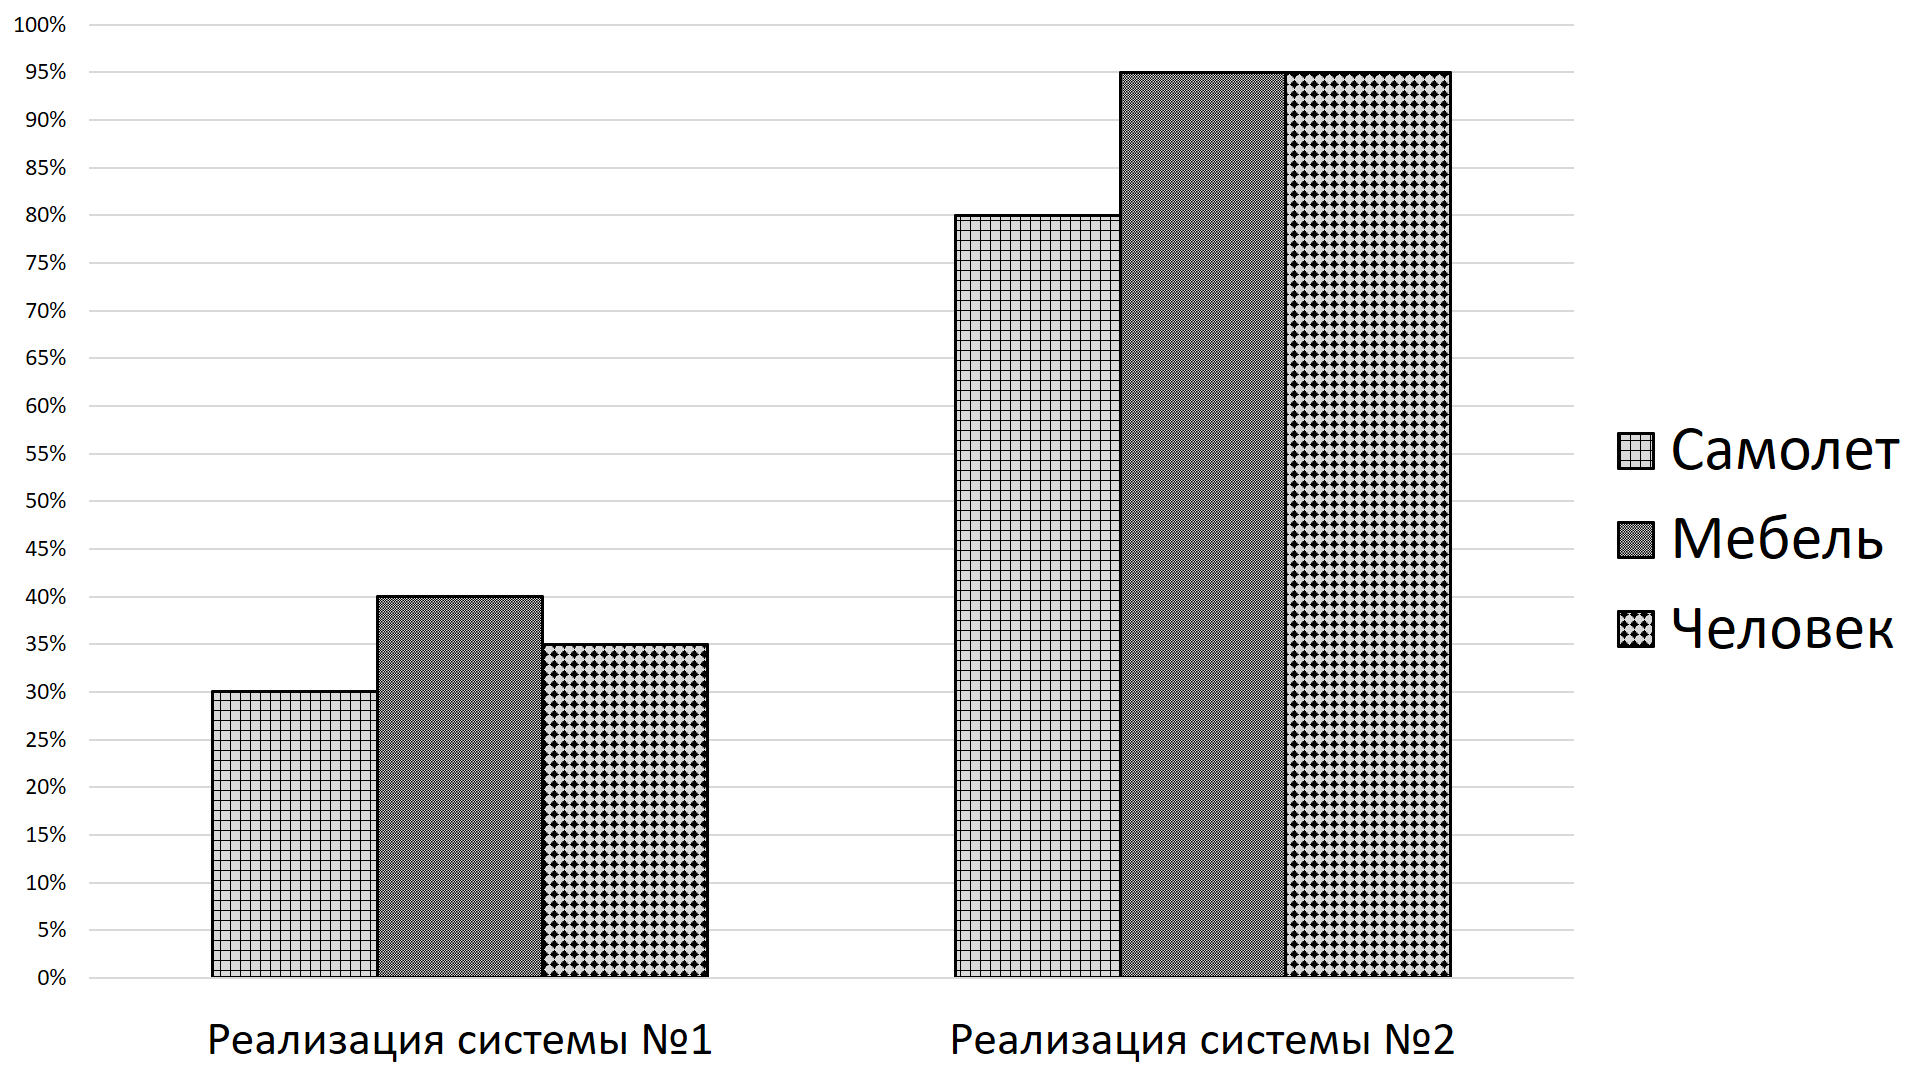
\includegraphics[scale=0.3] {13.JPG}
       \caption{Диаграмма результатов работы системы классификации трехмерных объектов}
       \label{ris:13}
   \end{center}
\end{figure}

Из данной диаграммы видно, что первая реализация системы не показала хороших результатов распознавания. В лучшем случае сеть смогла правильно классифицировать не более 40\% передаваемых ей объектов. Вторая же реализация системы показала наилучшие результаты из всех проведенных тестов. Качество распознавания в этом случае достигает 95\%.

\newpage
\addcontentsline{toc}{section}{Заключение}
\section*{Заключение}

В ходе работы была разработана система классификации трехмерных объектов. В процессе разработки данной системы были исследованы возможные представления (дескрипторы) трехмерных объектов, а также технологии сверточных нейронных сетей.

В ходе создания системы классификации трехмерных объектов были исследованы и реализованы алгоритмы подготовки моделей к построению глобальных дескрипторов формы поверхности в виде интегральных спиновых изображений, а также разработана и реализована сверточная нейронная сеть, классифицирующая объекты на три класса.

Анализируя результаты экспериментов можно сделать вывод, что предложенная система вполне способна выделять отличительные признаки трехмерных объектов не зависимо от их локальных различий в форме, масштаба и поворота в пространстве.

Основной проблемой при разработке подобной системы является большое количество варьируемых параметров на каждом ее этапе, а также малочисленность баз трехмерных объектов. В заключении стоит отметить, что полученный результат применения предложенной системы классификации при небольшом количестве трехмерных объектов дает предпосылки к тому, что при увеличении базы данных трехмерных моделей и вычислительной мощности, используемой для работы системы, возможно добиться корректных результатов распознавания данной системой для большого количества классов объектов.

\newpage
\addcontentsline{toc}{section}{Список литературы}
\bibliographystyle{utf8gost705u}  %% стилевой файл для оформления по ГОСТу
\begin{thebibliography}{9}

	\bibitem{Horn}
	Horn B. K. P. Extended Gaussian images // Proc. of the IEEE, 72, 1984, pp. 1671-1686

	\bibitem{Spin}
	Johnson A.E. Spin-Images: A Representation for 3-D Surface Matching, Ph. D. Thesis // Carnegie Mellon University, 1997, 288 p.

	\bibitem{Kang}
	Kang S. B. The complex EGI: A new representation for 3D pose determination / S. B. Kang, K. Ikeuchi // IEEE Trans. Pattern Anal. and Mach. Intell., 15(7), 1993, pp. 707-721

	\bibitem{Novotni}
	Novotni M. 3D zernike descriptors for content based shape retrieval / M. Novotni, R. Klein // In Proc. of the 8th ACM symposium on Solid modeling and applications (SM ’03), New York, NY, USA, ACM Press, 2003, pp. 216-225

	\bibitem{LeCun}
	LeCun, Yann. "LeNet-5, convolutional neural networks" –-- http://yann.lecun.com/exdb/lenet/

	\bibitem{Fukushima}
	Fukushima Kunihiko Neocognitron: A Self - organizing Neural Network Model for a Mechanism of Pattern Recognition Unaffected by Shift in Position. // Biological Cybernetics 1980 36 (4)

	\bibitem{Borisov1}
	Борисов Е. Базовые методы обработки изображений. // http://mechanoid.kiev.ua/cv-base.html

	\bibitem{Borisov2}
	Борисов Е. О методах обучения многослойных нейронных сетей прямого распространения. // http://mechanoid.kiev.ua/neural-net-backprop.html

	\bibitem{Stanford}
	CS231n: Convolutional Neural Networks for Visual Recognition. // http://cs231n.github.io

	\bibitem{LeCunBackProb}
	Y. LeCun, L. Bottou, G. Orr and K. Muller: Efficient BackProp, in Orr, G. and Muller K. (Eds), Neural Networks: Tricks of the trade, Springer, 1998

	\bibitem{Chernikoff}
	Черников И. Методы и алгоритмы реконструкции поиска и визуализации трехмерных моделей. - Воронежский государственный университет // Воронеж, 2013

\end{thebibliography}

\newpage
\addcontentsline{toc}{section}{Приложение А}
\label{attachA}\section*{Приложение А}

В данном приложении приведена реализация методов, которые отвечают за разделение ребер(edge-split) или их уничтожение(edge-collapse), в алгоритме контроля разрешения трехмерных объектов:

\lstinputlisting[language=C]{attach1.c}

\newpage
\addcontentsline{toc}{section}{Приложение Б}
\section*{Приложение Б}

В данном приложении приведена реализация архитектуры сверточной нейронной сети для классификации дескрипторов трехмерных объектов которой на вход передаются массивы размерности $[32 \times 32 \times 3]$.

 \lstinputlisting{attach2.m}

\newpage
\addcontentsline{toc}{section}{Приложение В}
\section*{Приложение В}

В данном приложении приведена реализация архитектуры сверточной нейронной сети для классификации дескрипторов трехмерных объектов которой на вход передаются массивы размерности $[28 \times 28]$.

\lstinputlisting{attach3.m}

%----------------------------------------------------------------------------------------

\end{document}
